\documentclass[a4paper, onehalfspacing, usecolor, 12pt]{bwthesisEN}
% The usecolor option sets the titles in blue, as requested by
% the Ghent University housestyle. Remove this to get a black
% and white version of things.
\usepackage[english]{babel} %Use dutch headings and titles

%-------------------------------------------------------------------------------
% FILL IN YOUR DETAILS
%
% Keep in mind that UGent doesn't use copromotors any longer. However,
% if it is required to add, please uncomment the line starting with
% \copromotor below and fill in the correct details.
%
\title{Hyperdimensional computing for protein language modeling}
\subtitle{...}
\author{Michael Fatjanov}

%\wordcount{6.431} % Fill in the number of words
\studentnr{...} % Fill in your student number

\promotor{Prof. Dr. Bernard De Baets}
\copromotor{Dr. Michiel Stock}
\tutor{Dimitri Boeckaerts}

\degree{master}
\richting{Bioinformatics}

\academicyear{2022 - 2023}

%-------------------------------------------------------------------------------
% The preamble. Note that the following packages are already loaded by
% the class bwthesis: geometry, amsmath, amsfonts, amssymb, graphicx,
% xcolor, ulem, setspace

% This package provides the lstlisting environment
\usepackage{listings}
\definecolor{mygreen}{rgb}{0,0.6,0}


\lstset{ %
	language=Python,                % choose the language of the code
	basicstyle=\footnotesize\ttfamily,       % the size of the fonts that are used for the code
	numbers=left,                   % where to put the line-numbers
	numberstyle=\scriptsize,      % the size of the fonts that are used for the line-numbers
	stepnumber=1,                   % the step between two line-numbers. If it is 1 each line will be numbered
	numbersep=5pt,                  % how far the line-numbers are from the code
	backgroundcolor=\color{white},  % choose the background color. You must add \usepackage{color}
	showspaces=false,               % show spaces adding particular underscores
	showstringspaces=false,         % underline spaces within strings
	showtabs=false,                 % show tabs within strings adding particular underscores
	frame=none,           % adds a frame around the code
	tabsize=2,          % sets default tabsize to 2 spaces
	captionpos=b,           % sets the caption-position to bottom
	breaklines=true,        % sets automatic line breaking
	breakatwhitespace=false,    % sets if automatic breaks should only happen at whitespace
	xleftmargin=15pt,
	xrightmargin=5pt,
	commentstyle=\color{mygreen}, %teal
	keywordstyle=\color{blue},
	stringstyle=\color{orange}       % if you want to add LaTeX within your code
} % contains settings for the package listings
% this package provides an environment for algorithms (cfr. Pseudocode)
\usepackage[ruled]{algorithm2e} 
% This package provides extra possibilities for tables
\usepackage{booktabs}
% this package is used to produce both author-date and standard numerical citations for BibTeX bibliographies
\usepackage[round]{natbib}
% This packages adds the Appendix name in the toc. See below
\usepackage[titletoc]{appendix}

% ---- ADDITIONAL SETTINGS
\graphicspath{{Fig/}} % path to the figure directory

%-------------------------------------------------------------------------------
% The actual document
%
\begin{document}


% Typisch copyright voor een thesis.
% Te plaatsen juist na het titelblad.
% De namen worden automatisch ingevuld, maar 

\par\vspace*{\fill}

De auteur en promotor geven de toelating deze scriptie voor consultatie beschikbaar te stellen en delen ervan te kopi\"eren voor persoonlijk gebruik. Elk ander gebruik valt onder de beperkingen van het auteursrecht, in het bijzonder met betrekking tot de verplichting uitdrukkelijk de bron te vermelden bij het aanhalen van resultaten uit deze scriptie.

The author and promoter give the permission to use this thesis for consultation and to copy parts of it for personal use. Every other use is subject to the copyright laws, more specifically the source must be extensively specified when using results from this thesis.

\vspace{1cm}

Gent, FILL IN THE DATE % FILL IN THE CORRECT DATE

\vspace{1cm}

\begin{minipage}[t][4cm][t]{0.5\textwidth}
\raggedright
The promotor,

\vspace{2.5cm}

\insertpromotor % Change if multiple names are necessary
\end{minipage}
\begin{minipage}[t][4cm][t]{0.48\textwidth}
\raggedright
The author,

\vspace{2.5cm}

\insertauthor % change if your name should be different
\end{minipage}

\thispagestyle{empty} 


\clearpage{\pagestyle{empty}\cleardoublepage}

%------------------------------------------------------------------------
\frontmatter
\pagestyle{frontmatter} %sets headers and footers correctly

% ------------ thanks -----------
\chapter{Acknowledgements}
I am sincerely grateful to my supervisor, ir. D. Boeckaerts, whose commitment to my project extended to countless proofreadings and always being on hand to answer my relentless questions. Your guidance and dedication have been invaluable and created an enjoyable and engaging learning experience.

I would also like to extend my gratitude to my promoters, Prof. B. De Baets and dr. ir. M. Stock, who made this work possible to begin with and contributed to this work by collectively proofreading my dissertation and providing insightful ideas and suggestions. Their combined expertise, keen attention to detail, and valuable feedback have significantly elevated the quality of this work.

I must also express my heartfelt gratitude to my partner, who has provided much support and encouragement throughout this journey. Your understanding and emotional support have made this challenging process much more manageable.

To my classmates, thank you for the frequent companions of coffee machine banter. The camaraderie, discussions, and shared laughter we experienced brought light to even the most stressful of days.

Lastly, my thanks go to my family. Your ongoing support and encouragement have been greatly appreciated. Thank you for everything.

% ------------ table of contents ---------
{
	\singlespacing % to keep the TOC within boundaris
  % Remove whitespace between the sections
  \setlength{\parskip}{0ex plus 0.3ex minus 0.3ex}
	\tableofcontents
}

\addcontentsline{toc}{chapter}{Contents} %add TOC to the TOC


% ------------ summary ----------
\chapter[Nederlandse samenvatting]{Samenvatting}

nederlandse samenvatting





\chapter{Abstract}
This dissertation explores the implementation and application of hyperdimensional computing for protein sequence analysis. We discuss the advancements of state-of-the-art protein language models in protein structure and function predictions while raising the need for more computationally and data-efficient methods. As hyperdimensional computing is proposed as a promising avenue, its underlying principles and mathematical operations are illustrated to demonstrate the potential of hyperdimensional computing in bioinformatics research. 

We research and develop several methods to encode amino acids into hyperdimensional vectors. Of these, projecting embeddings containing biological information into hyperdimensional space has proven to be useful in subsequent analyses and prediction tasks. Utilizing the PhaLP database~\cite{phalp}, a continuously updated database of phage lytic proteins, we apply these amino acid encoding methods to develop techniques for protein sequence encodings. We demonstrate the capability of these methods to capture essential protein sequence information in hyperdimensional vectors, proving their usefulness in prediction tasks. In our classification tasks, we show that hyperdimensional-computing-based learning methods display competitive performance when compared to established machine learning methods such as random forest and XGBoost. In addition, we examine perceptron-based models for context-aware protein residue learning, utilizing neighborhood-encoded hyperdimensional vectors. Although this does not outperform current state-of-the-art models, it contributes valuable insights into the challenges faced when implementing efficient models for such tasks within the hyperdimensional computing framework. 

Finally, we acknowledge the need for continued research in refining our encoding algorithms, exploring alternative model architectures, and extending the scope of tasks and datasets. Despite mixed results, our findings lay a solid foundation for further investigation into hyperdimensional computing's potential in protein sequence research and bioinformatics.

% The following can be commented out to remove the list of figures
% and the list of tables, as specified by the guidelines of BW
% \listoffigures
% \listoftables

%-----------------------------------------------------------------------
\mainmatter
\pagestyle{mainmatter} % sets headers and footers correctly

% Here you can add more chapters in case it is needed
\chapter[Introduction]%
{Introduction}
%% Introduction
%%%%%%%%%%%%%%%
\section{Big picture and traditional bioinformatics tools for protein research}
Proteins are an essential part of molecular biology and are responsible for a wide variety of functions. Far too wide to discuss here because they are one of the building blocks that make up life, hence a lot of effort has gone towards trying to understand the functions of protein and disruptions in its mechanisms that lead to many kinds of diseases. In spite of that, for a large fraction of the approximately 20000 human proteins, the structures and functions remain still unknown. To start, proteins are composed of a linear chain of amino acids (AA) with a length ranging from 50 to tens of thousands of AAs, all connected by peptide bonds into a polypeptide. This is also referred to as the \textit{primary structure} of a protein.\cite{primstruct} A sequence of amino acids is mostly determined by the genetic code without considering post-translational and post-transcriptional modifications etc. In the genetic code of all living organisms, there are 20 different kinds of amino acids coded which make up the 'language' of proteins. The current state-of-the-art methods for the identification of protein sequences are \textit{de novo sequencing} algorithms applied to tandem mass spectrometry data.\cite{protseq}

It is intuitive to represent a protein as a sequence of letters with each letter corresponding to an amino acid. Likewise to natural languages, we can find common elements between naturally evolved proteins. These motifs and domains are essential to many biological processes and can easily be represented as words, phrases and sentences of amino acids.
A traditional task in bioinformatics and more specifically in the realm of protein sequence analyses is the quantification of the similarity between strings of sequences. Classical pairwise alignment algorithms include the algorithm of \textbf{Needleman \& Wunsch} \cite{global} for global alignments and that of \textbf{Smith \& Waterman} \cite{local} for local alignments. These algorithms are sufficient for comparing two sequences but unfeasible for searching databases for homologous sequences, hence faster algorithms like FASTA \cite{fasta} and, as of yet widely used for simple searches for similar sequences, BLAST \cite{blast} were made. A natural extension of pairwise alignment is multiple sequence alignment (MSA), which is to align multiple related sequences. This reveals much more information than pairwise alignment can. It allows for the identification of conserved sequence patterns and critical amino acid residues which is highly important for constructing phylogenetic profiles and can help in the prediction of secondary and tertiary 3-dimensional structures as we see later.

To cope with the number of recorded protein sequences rising exponentially, far more compute-wise efficient methods based on multiple sequence alignments had to be developed like PSI-BLAST \cite{psiblast}, HHblits \cite{hhblits3} and MMseqs \cite{mmseqs2}. However, these methods might not be able to keep up with the ever increasing number of protein sequences stored in databases.

A protein also consists of much more than a mere sequence, however. It is a 3-dimensional structure with a predetermined form and function. While a protein's structure and function are dynamic and dependent on its surroundings such as the cellular state and other proteins and molecules akin to natural languages, it is still defined by its underlying sequence. This means that a lot of the 3D-structural and functional information of a protein should be retrievable from its amino acid sequence.\cite{structure} The most common way to determine the 3D structure of a protein has remained to be X-ray crystallography for more than half a century \cite{xray}, with cyro-electron microscopy now catching up rapidly.\cite{cyroem} However, these kinds of laboratory approaches for structure determination of proteins are not simple, expensive and in some cases not possible for the protein in question whilst sequence determination is relatively much easier to perform.For this reason, the number of verified three-dimensional structures has not kept up with the explosive growth in sequence information. On top of that, structure prediction is highly in demand for researchers in applications such as drug design.  Therefore, a lot of effort has gone into computational methods for structure and function predictions from protein sequences.

\section{State-of-the-art protein language modeling}

\section{Hyperdimensional computing}
Hyperdimensional computing (HDC) is a relatively new paradigm of computing developed by \textbf{Kanerva} \cite{Kanerva2009} that tries to mimic the workings of a (human) brain by computing with vectors of tens of thousands of elements long, so in the realm of hyperdimensionality. The human brain consists of about 100 billion neurons (nerve cells) and 1000 trillion synapses that connect these neurons. Each neuron is connected to up to 10000 other neurons, creating massive circuits. This is likely fundamental to the workings of the human brain and what separates our brains from modern von Neumann computer architectures which operate on 8 to 64-bit vectors. This becomes clear when we compare the relative simplicity for a human to learn a language compared to computers. Computers use a large and complicated set of arithmetic operations in the form of deep learning networks which require terabytes of data and thousands of Watts of computing power to come close to mastering a language whilst a human can recognize other languages relatively easily when they don't even speak it. Likewise languages, we can very easily memorize and compare other intrinsically complex and contextual concepts such as images. A computer would have a hard time finding similarities between a set of images and faces because this requires very complex machine learning models. The human brain can do this all with a very large efficiency by consuming only roughly 20 W of energy.

Achieving these kinds of flexible brain-like models based on high dimensionality is not entirely new and is being explored since the 1990s. Some of these earlier models include Holographic Reduced Representations~\cite{HRR}, Spatter Code~\cite{spatter} etc. A hyperdimensional vector (HDV) can represent anything from a scalar number to any kind of concept. This vector is initially made up of totally random elements, but with a simple set of operations which will be explained later, we can use other vectors to combine some concepts into new similar or dissimilar concepts. For example, to show the essence of HDC and how it tries to simulate the brain, we can compare the concept of a \textit{table} to the concept of a \textit{brocolli}. We would not immediately conclude that they are in any way similar but as humans, we can trace back \textit{table} to \textit{plate} which has some similarities with \textit{food} from which we can easily extract the concept of \textit{brocolli}. These kinds of operations are not very obvious for a classical computer but creating these semantic pathways are rather easy for humans.

The elements in an HDV can be made up of binary bits like in classical computing but also of bipolar or real numbers. The choice of the nature of the elements has also implications on the nature of the different operations and the results. Highly efficient bit operations could be used on binary vectors but then the amount of information stored in such a vector would be drastically lessened compared to bipolar or real vectors, leading to lower accuracy.  

An initial HDV is made up fully randomly. This \textit{holistic} or \textit{holographic} representation of a concept smeared out over a vector consisting of thousands of bits gives rise to interesting properties such as its robustness. These kinds of systems are very tolerant to noise and failure of bits since we introduce a lot of redundancy in the vector just by stochastics. This is very unlike classical computing where every bit counts and one failure in a bit can lead to disasters. 
\subsection{Operations on hyperdimensional vectors}
The interesting properties of HDC are based on only four basic operations we can perform on HDVs. We will discuss these for bipolar and binary vectors.
\subsubsection{Similarity measurement} \label{sssec:sim}
For many kinds of problems, it will be necessary to quantify the similarity between two HDVs. The method depends on the nature of the vectors. For binary vectors, the \textit{Hamming distance} defined as in equation~\ref{eqn:Hamming} is widely used.
\begin{equation}
    \label{eqn:Hamming}
    Ham(A, B) = \frac{1}{d} \sum_{i=1}^{d} 1_{A_{(i)} \neq B_{(i)}}
\end{equation}
The \textit{cosine distance} as defined in equation~\ref{eqn:cosine} is most commonly used for bipolar vectors.
\begin{equation}
    \label{eqn:cosine}
    cos(A, B) = \frac{A \cdot B}{||A|| * ||B||}
\end{equation}
The results of both of these measurements are summarized in table~\ref{tab:dist}.
\begin{table}[h]
    \begin{tabular}{|c||c|c|c|}
        \hline
        \textbf{Measurement} & \textbf{Dissimilar} & \textbf{Orthogonal} & \textbf{Similar} \\
        \hline
        \textbf{Hamming distance} & 1 & 0.5 & 0 \\
        \hline
        \textbf{Cosine similarity} & -1 & 0 & 1 \\
        \hline
    \end{tabular}
    \caption{\label{tab:dist}Overview of similarity measurements in HDC depending on the nature of the HDVs} 
\end{table}
It is important to note that two random HDVs will be orthogonal to each other just by stochastics. Also notice that the first quantifies a distance and the latter a similarity.
\subsubsection{Addition} \label{sssec:add}
Also referred to as \textit{bundling}, the element-wise addition as in equation~\ref{eqn:sum} of $n$ input vectors $\{X_{1} + X_{2} + \cdots + X_{n}\}$ creates a vector $X$ that is maximally similar to the input vectors.
\begin{equation}
    \label{eqn:sum}
    X = X_{1} + X_{2} + \cdots + X_{n}
\end{equation}
For bipolar vectors this is straightforward. The input vectors are added element-wise but the resulting vector is restricted to a bipolar nature too depending on the sign of each element, thus containing only $-1$, $1$ but allowing $0$ for elements that are in disagreement as shown in the following $6$-dimensional example.
\begin{alignat*}{7}
    X_{1} &= && \qquad +1 && \qquad -1 && \qquad +1 && \qquad +1 && \qquad -1 && \qquad -1 \\
    X_{2} &= && \qquad +1 && \qquad +1 && \qquad +1 && \qquad -1 && \qquad -1 && \qquad -1 \\
    X_{3} &= && \qquad -1 && \qquad -1 && \qquad +1 && \qquad +1 && \qquad -1 && \qquad +1 \\
    X_{4} &= && \qquad -1 && \qquad -1 && \qquad -1 && \qquad +1 && \qquad -1 && \qquad +1 \\
    \hline
    X_{1} + X_{2} + X_{3} + X_{4} &= && \qquad \phantom{-}0 && \qquad -1 && \qquad +1 && \qquad +1 && \qquad -1 && \qquad \phantom{-}0
\end{alignat*}
For binary vectors, the vectors are element-wise bundled based on the majority element. This is no problem if an odd number of input vectors are considered but ambiguity rises when bundling an even set of vectors. This can be solved by setting the element in question randomly.~\cite{binBund} Another possibility is to add another random vector however this may seem to add more unnecessary noise, especially when bundling a low number of vectors. We can also reverse this by an \textit{inverse addition}. For bipolar vectors, this means just multiplying the vector of interest by -1. A binary vector can be flipped bit-wise.

Similar to an ordinary arithmetic summation, the bundling addition of hyperdimensional vectors is commutative so the result is not dependent on the order of addition.
\begin{equation}
    \label{eqn:sumcom}
    X_{1} + X_{2} = X = X_{2} + X_{1}
\end{equation}
\subsubsection{Multiplication} \label{sssec:mult}
Also referred to as \textit{binding}, we can element-wise multiply two vectors resulting in a vector maximally dissimilar to the input vectors. Vectors $X$ and $Y$ are bound together forming $Z$ being orthogonal to $X$ and $Y$ as shown in equation~\ref{eqn:multp}.
\begin{equation}
    \label{eqn:multp}
    Z = X * Y
\end{equation}
This \textit{binding} operation translates to a simple arithmetic element-wise multiplication for bipolar vectors. For binary vectors, this is represented by a \textit{XOR} bit-operation shown as follows.
\begin{alignat*}{7}
    X &= && \qquad 1 && \qquad 0 && \qquad 1 && \qquad 1 && \qquad 0 && \qquad 0 \\
    Y &= && \qquad 1 && \qquad 1 && \qquad 0 && \qquad 1 && \qquad 0 && \qquad 1 \\
    \hline
    X * Y &= && \qquad 0 && \qquad 1 && \qquad 1 &&  \qquad 0 && \qquad 0 && \qquad 1 \phantom{-}0
\end{alignat*}
This operation can also be undone by multiplying with the same vector again. It is its own inverse so that
\begin{equation}
    \label{eqn:multpinv}
    A * A = O \text{ where $O$ is a vector containing only 0s}
\end{equation}
Likewise an ordinary multiplication, this operation is commutative and distributive over additions, meaning that transforming a bundle of concepts with binding is equivalent to binding every element before bundling.
\begin{equation}
    \label{eqn:multpdis}
    A = Z*(X + Y) = XZ + YZ
\end{equation}
\subsubsection{Permutation} \label{sssec:perm}
The permutation operation of an HDV, also known as \textit{shifting}, is a simple reordering of the HDV. This can be random but a circular shift is widely employed~\cite{HD_rev} and makes the operation easily reversible. This results in a vector technically dissimilar from the input vector but still encoding its information. This will become important later when it will be used to encode sequential information such as tokens in a text. This operation will be denoted by $\Pi$.
\begin{alignat*}{7}
    X &= && \qquad 1 && \qquad 0 && \qquad 1 && \qquad 1 && \qquad 0 && \qquad 0 \\
    \hline
    \Pi(X) &= && \qquad 0 && \qquad 1 && \qquad 0 &&  \qquad 1 && \qquad 1 && \qquad 0
\end{alignat*}
\subsection{Examples}
There are many interesting possibilities given the relative simplicity of all these operations. We shall illustrate some applications and examples. 
In the following example, the robustness of these hyperdimensional vectors is shown. Assume $A, B, C, X, Y, Z$ to be random 10000-dimensional bipolar hypervectors and $D = X*A + Y*B + Z*C$. We will try to retrieve A from D.
\begin{align}
    \label{eqn:ex1}
    A' &= X * D \\
    &= X * (X * A + Y * B + Z * C) \\
    &= \underbrace{X * X * A}_A + \underbrace{X * Y * B + X * Z * C}_\text{noise} \\
    &\approx A
\end{align}
This example was implemented in a Julia script, the results are illustrated in figure~\ref{fig:exm1}.
\begin{figure}[h]
    \centering
    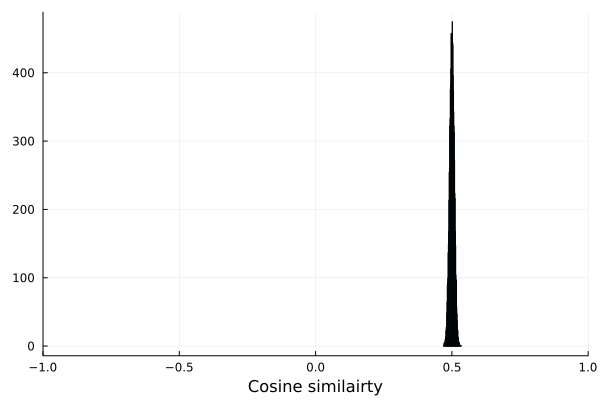
\includegraphics[scale = 0.7]{showcase}
    \caption{10000 cases of random 10000-dimensional bipolar vectors are made and each time implemented following example~\ref{eqn:ex1}. The resulting cosine similarities between $A$ and $A'$ are then plotted in a histogram.}
    \label{fig:exm1}
\end{figure}

We see that we can retrieve a lot of information with most of the cosine similarities centering around 0.5. Notice that two completely random HDVs would have a cosine similarity close to 0 just by stochastics. This result is not comparable to state-of-the-art accuracies but very efficient nonetheless as all of these calculations were done in less than 2 seconds. This same experiment was done with random binary 10000-dimensional vectors and it finished even faster as expected but retained the accuracy (similar \textit{Hamming distance} peak around 0.25).

% ------------ REFERENCES ------------
% Here you have your bibliography created


\addcontentsline{toc}{chapter}{Bibliography} %show bibliography in TOC
\bibliographystyle{apalike}  %apalike,phdbib.bst
\bibliography{Thesis_bib}

% Here you insert your appendices
\appendix

\begin{appendices}

% Dit voegt het woord Bijlage toe aan de titel!
\titleformat{\chapter} % command
  [display] % shape
  {\fontsize{18}{22} \selectfont \coltitle } % format
  {\MakeUppercase{\chaptertitlename \ \thechapter}} % the label
  {-2ex} %separator space
  {\fontsize{24}{32} \selectfont \bf \raggedright \MakeUppercase{\uline{#1}}} %before code
  { } %aft%after code


\chapter{Additional information on Chapter 3}\label{app:chp3}
\begin{figure}[h!]
    \centering
    \begin{subfigure}{0.48\textwidth}
        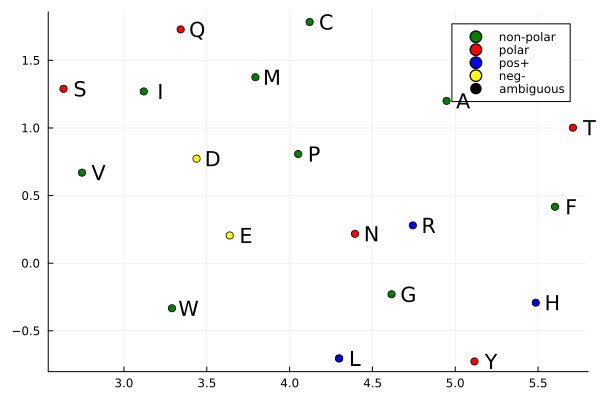
\includegraphics[width=\textwidth]{ur4tr_emb}
        \caption{Made starting from random hyperdimensional vectors for each amino acid, $k=4$.}
        \label{fig:AAtr4ru}
    \end{subfigure}
    \hfill
    \begin{subfigure}{0.48\textwidth}
        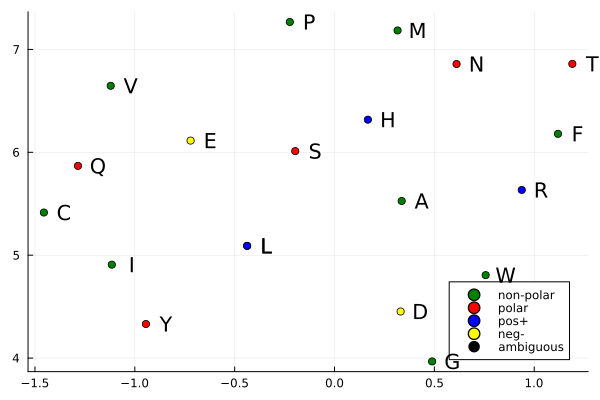
\includegraphics[width=\textwidth]{ur50tr_emb}
        \caption{Made starting from random hyperdimensional vectors for each amino acid, $k=50$.}
        \label{fig:AAtr50ru}
    \end{subfigure}
    
    \begin{subfigure}{0.48\textwidth}
        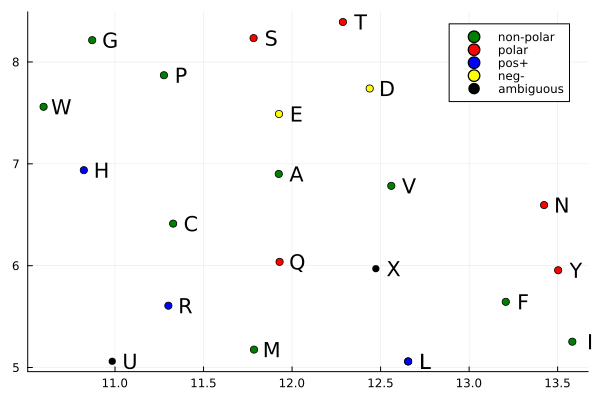
\includegraphics[width=\textwidth]{u4tr_emb}
        \caption{Made starting from extended ESM-2 embeddings for each amino acid, $k=4$.}
        \label{fig:AAtr4u}
    \end{subfigure}
    \hfill
    \begin{subfigure}{0.48\textwidth}
        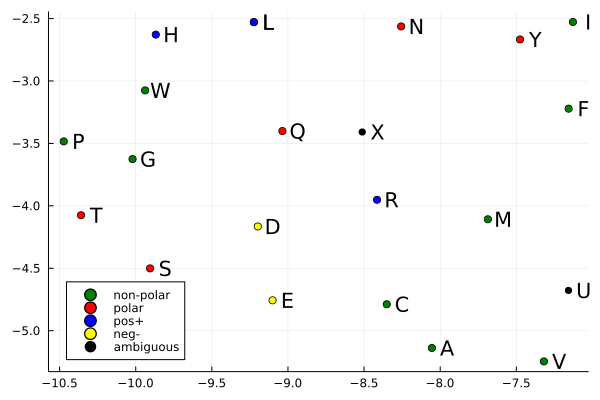
\includegraphics[width=\textwidth]{u50tr_emb}
        \caption{Made starting from extended ESM-2 embeddings for each amino acid, $k=50$.}
        \label{fig:AAtr50u}
    \end{subfigure}
    \caption{Scatter plot of a two-dimensional UMAP projection of the average amino acid HDVs with neighborhood-information of $k$ encoded. Learned from the human reference proteome. The amino acids are annotated and colored based on their chemical property of polarity.}
    \label{fig:main3}
\end{figure}

\begin{table}[h!]
    \label{tbl:target_grant}
    \caption{Target similarities made from Grantham's distance matrix}
    \resizebox{\textwidth}{!}{\begin{tabular}{cccccccccccccccccccc}
        $0.0$ & $0.73$ & $0.87$ & $0.8$ & $0.87$ & $0.73$ & $0.87$ & $0.8$ & $0.8$ & $0.8$ & $0.8$ & $0.87$ & $0.8$ & $0.8$ & $0.8$ & $0.67$ & $0.73$ & $0.73$ & $0.93$ & $0.87$\\ \hline
        $0.73$ & $0.0$ & $0.93$ & $1.0$ & $0.87$ & $0.93$ & $0.93$ & $0.8$ & $0.93$ & $0.8$ & $0.8$ & $0.93$ & $0.93$ & $0.93$ & $0.93$ & $0.8$ & $0.8$ & $0.8$ & $0.87$ & $0.87$\\ \hline
        $0.87$ & $0.93$ & $0.0$ & $0.6$ & $0.93$ & $0.8$ & $0.8$ & $0.93$ & $0.8$ & $1.0$ & $0.93$ & $0.67$ & $0.8$ & $0.73$ & $0.87$ & $0.73$ & $0.8$ & $0.93$ & $1.0$ & $0.93$\\ \hline
        $0.8$ & $1.0$ & $0.6$ & $0.0$ & $0.93$ & $0.87$ & $0.73$ & $0.93$ & $0.67$ & $0.93$ & $0.87$ & $0.73$ & $0.8$ & $0.6$ & $0.73$ & $0.73$ & $0.8$ & $0.87$ & $0.93$ & $0.87$\\ \hline
        $0.87$ & $0.87$ & $0.93$ & $0.93$ & $0.0$ & $0.93$ & $0.8$ & $0.73$ & $0.93$ & $0.73$ & $0.73$ & $0.93$ & $1.0$ & $0.93$ & $0.93$ & $0.87$ & $0.87$ & $0.8$ & $0.67$ & $0.53$\\ \hline
        $0.73$ & $0.93$ & $0.8$ & $0.87$ & $0.93$ & $0.0$ & $0.87$ & $1.0$ & $0.87$ & $1.0$ & $0.93$ & $0.73$ & $0.87$ & $0.87$ & $0.87$ & $0.73$ & $0.87$ & $0.93$ & $0.87$ & $0.93$\\ \hline
        $0.87$ & $0.93$ & $0.8$ & $0.73$ & $0.8$ & $0.87$ & $0.0$ & $0.93$ & $0.8$ & $0.93$ & $0.87$ & $0.67$ & $0.87$ & $0.73$ & $0.73$ & $0.8$ & $0.87$ & $0.93$ & $0.87$ & $0.6$\\ \hline
        $0.8$ & $0.8$ & $0.93$ & $0.93$ & $0.73$ & $1.0$ & $0.93$ & $0.0$ & $0.93$ & $0.6$ & $0.67$ & $0.93$ & $0.93$ & $0.93$ & $0.93$ & $0.87$ & $0.8$ & $0.53$ & $0.93$ & $0.8$\\ \hline
        $0.8$ & $0.93$ & $0.8$ & $0.67$ & $0.93$ & $0.87$ & $0.8$ & $0.93$ & $0.0$ & $0.87$ & $0.8$ & $0.73$ & $0.8$ & $0.67$ & $0.6$ & $0.73$ & $0.8$ & $0.87$ & $0.93$ & $0.87$\\ \hline
        $0.8$ & $0.8$ & $1.0$ & $0.93$ & $0.73$ & $1.0$ & $0.93$ & $0.6$ & $0.87$ & $0.0$ & $0.6$ & $0.93$ & $0.93$ & $0.87$ & $0.87$ & $0.87$ & $0.8$ & $0.67$ & $0.87$ & $0.8$\\ \hline
        $0.8$ & $0.8$ & $0.93$ & $0.87$ & $0.73$ & $0.93$ & $0.87$ & $0.67$ & $0.8$ & $0.6$ & $0.0$ & $0.87$ & $0.87$ & $0.73$ & $0.8$ & $0.8$ & $0.8$ & $0.67$ & $0.8$ & $0.8$\\ \hline
        $0.87$ & $0.93$ & $0.67$ & $0.73$ & $0.93$ & $0.73$ & $0.67$ & $0.93$ & $0.73$ & $0.93$ & $0.87$ & $0.0$ & $0.87$ & $0.73$ & $0.73$ & $0.67$ & $0.73$ & $0.93$ & $1.0$ & $0.87$\\ \hline
        $0.8$ & $0.93$ & $0.8$ & $0.8$ & $1.0$ & $0.87$ & $0.87$ & $0.93$ & $0.8$ & $0.93$ & $0.87$ & $0.87$ & $0.0$ & $0.8$ & $0.87$ & $0.8$ & $0.8$ & $0.87$ & $1.0$ & $0.93$\\ \hline
        $0.8$ & $0.93$ & $0.73$ & $0.6$ & $0.93$ & $0.87$ & $0.73$ & $0.93$ & $0.67$ & $0.87$ & $0.73$ & $0.73$ & $0.8$ & $0.0$ & $0.67$ & $0.73$ & $0.8$ & $0.87$ & $0.87$ & $0.8$\\ \hline
        $0.8$ & $0.93$ & $0.87$ & $0.73$ & $0.93$ & $0.87$ & $0.73$ & $0.93$ & $0.6$ & $0.87$ & $0.8$ & $0.73$ & $0.87$ & $0.67$ & $0.0$ & $0.8$ & $0.8$ & $0.93$ & $0.93$ & $0.87$\\ \hline
        $0.67$ & $0.8$ & $0.73$ & $0.73$ & $0.87$ & $0.73$ & $0.8$ & $0.87$ & $0.73$ & $0.87$ & $0.8$ & $0.67$ & $0.8$ & $0.73$ & $0.8$ & $0.0$ & $0.67$ & $0.87$ & $0.93$ & $0.87$\\ \hline
        $0.73$ & $0.8$ & $0.8$ & $0.8$ & $0.87$ & $0.87$ & $0.87$ & $0.8$ & $0.8$ & $0.8$ & $0.8$ & $0.73$ & $0.8$ & $0.8$ & $0.8$ & $0.67$ & $0.0$ & $0.73$ & $0.87$ & $0.87$\\ \hline
        $0.73$ & $0.8$ & $0.93$ & $0.87$ & $0.8$ & $0.93$ & $0.93$ & $0.53$ & $0.87$ & $0.67$ & $0.67$ & $0.93$ & $0.87$ & $0.87$ & $0.93$ & $0.87$ & $0.73$ & $0.0$ & $0.93$ & $0.8$\\ \hline
        $0.93$ & $0.87$ & $1.0$ & $0.93$ & $0.67$ & $0.87$ & $0.87$ & $0.93$ & $0.93$ & $0.87$ & $0.8$ & $1.0$ & $1.0$ & $0.87$ & $0.93$ & $0.93$ & $0.87$ & $0.93$ & $0.0$ & $0.6$\\ \hline
        $0.87$ & $0.87$ & $0.93$ & $0.87$ & $0.53$ & $0.93$ & $0.6$ & $0.8$ & $0.87$ & $0.8$ & $0.8$ & $0.87$ & $0.93$ & $0.8$ & $0.87$ & $0.87$ & $0.87$ & $0.8$ & $0.6$ & $0.0$
        \end{tabular}}
\end{table}

\begin{table}[h!]
    \label{tbl:achieved_grant}
    \caption{Achieved similarities targeting Grantham's distance matrix}
    \resizebox{\textwidth}{!}{\begin{tabular}{cccccccccccccccccccc}
        $0.0$ & $0.49$ & $0.49$ & $0.48$ & $0.48$ & $0.49$ & $0.5$ & $0.49$ & $0.49$ & $0.5$ & $0.49$ & $0.49$ & $0.49$ & $0.49$ & $0.49$ & $0.48$ & $0.5$ & $0.51$ & $0.49$ & $0.49$\\ \hline
$0.49$ & $0.0$ & $0.49$ & $0.5$ & $0.49$ & $0.49$ & $0.49$ & $0.5$ & $0.5$ & $0.48$ & $0.5$ & $0.5$ & $0.5$ & $0.49$ & $0.48$ & $0.49$ & $0.49$ & $0.49$ & $0.49$ & $0.49$\\ \hline
$0.49$ & $0.49$ & $0.0$ & $0.49$ & $0.49$ & $0.49$ & $0.49$ & $0.49$ & $0.49$ & $0.5$ & $0.49$ & $0.49$ & $0.5$ & $0.49$ & $0.49$ & $0.5$ & $0.49$ & $0.5$ & $0.49$ & $0.49$\\ \hline
$0.48$ & $0.5$ & $0.49$ & $0.0$ & $0.49$ & $0.48$ & $0.5$ & $0.5$ & $0.49$ & $0.49$ & $0.49$ & $0.5$ & $0.5$ & $0.5$ & $0.49$ & $0.5$ & $0.49$ & $0.49$ & $0.49$ & $0.49$\\ \hline
$0.48$ & $0.49$ & $0.49$ & $0.49$ & $0.0$ & $0.5$ & $0.5$ & $0.5$ & $0.49$ & $0.49$ & $0.5$ & $0.5$ & $0.5$ & $0.49$ & $0.5$ & $0.5$ & $0.51$ & $0.51$ & $0.5$ & $0.49$\\ \hline
$0.49$ & $0.49$ & $0.49$ & $0.48$ & $0.5$ & $0.0$ & $0.5$ & $0.49$ & $0.5$ & $0.49$ & $0.49$ & $0.5$ & $0.49$ & $0.49$ & $0.49$ & $0.5$ & $0.5$ & $0.49$ & $0.5$ & $0.5$\\ \hline
$0.5$ & $0.49$ & $0.49$ & $0.5$ & $0.5$ & $0.5$ & $0.0$ & $0.5$ & $0.51$ & $0.5$ & $0.5$ & $0.5$ & $0.5$ & $0.49$ & $0.49$ & $0.49$ & $0.49$ & $0.5$ & $0.48$ & $0.49$\\ \hline
$0.49$ & $0.5$ & $0.49$ & $0.5$ & $0.5$ & $0.49$ & $0.5$ & $0.0$ & $0.48$ & $0.49$ & $0.49$ & $0.51$ & $0.5$ & $0.5$ & $0.49$ & $0.5$ & $0.49$ & $0.5$ & $0.5$ & $0.5$\\ \hline
$0.49$ & $0.5$ & $0.49$ & $0.49$ & $0.49$ & $0.5$ & $0.51$ & $0.48$ & $0.0$ & $0.5$ & $0.49$ & $0.5$ & $0.5$ & $0.49$ & $0.5$ & $0.5$ & $0.48$ & $0.49$ & $0.49$ & $0.49$\\ \hline
$0.5$ & $0.48$ & $0.5$ & $0.49$ & $0.49$ & $0.49$ & $0.5$ & $0.49$ & $0.5$ & $0.0$ & $0.5$ & $0.5$ & $0.49$ & $0.49$ & $0.49$ & $0.49$ & $0.49$ & $0.5$ & $0.5$ & $0.48$\\ \hline
$0.49$ & $0.5$ & $0.49$ & $0.49$ & $0.5$ & $0.49$ & $0.5$ & $0.49$ & $0.49$ & $0.5$ & $0.0$ & $0.49$ & $0.49$ & $0.51$ & $0.5$ & $0.49$ & $0.5$ & $0.5$ & $0.49$ & $0.49$\\ \hline
$0.49$ & $0.5$ & $0.49$ & $0.5$ & $0.5$ & $0.5$ & $0.5$ & $0.51$ & $0.5$ & $0.5$ & $0.49$ & $0.0$ & $0.5$ & $0.49$ & $0.5$ & $0.49$ & $0.5$ & $0.49$ & $0.5$ & $0.49$\\ \hline
$0.49$ & $0.5$ & $0.5$ & $0.5$ & $0.5$ & $0.49$ & $0.5$ & $0.5$ & $0.5$ & $0.49$ & $0.49$ & $0.5$ & $0.0$ & $0.49$ & $0.5$ & $0.49$ & $0.5$ & $0.49$ & $0.5$ & $0.48$\\ \hline
$0.49$ & $0.49$ & $0.49$ & $0.5$ & $0.49$ & $0.49$ & $0.49$ & $0.5$ & $0.49$ & $0.49$ & $0.51$ & $0.49$ & $0.49$ & $0.0$ & $0.49$ & $0.5$ & $0.5$ & $0.5$ & $0.49$ & $0.5$\\ \hline
$0.49$ & $0.48$ & $0.49$ & $0.49$ & $0.5$ & $0.49$ & $0.49$ & $0.49$ & $0.5$ & $0.49$ & $0.5$ & $0.5$ & $0.5$ & $0.49$ & $0.0$ & $0.49$ & $0.49$ & $0.49$ & $0.5$ & $0.5$\\ \hline
$0.48$ & $0.49$ & $0.5$ & $0.5$ & $0.5$ & $0.5$ & $0.49$ & $0.5$ & $0.5$ & $0.49$ & $0.49$ & $0.49$ & $0.49$ & $0.5$ & $0.49$ & $0.0$ & $0.49$ & $0.5$ & $0.49$ & $0.5$\\ \hline
$0.5$ & $0.49$ & $0.49$ & $0.49$ & $0.51$ & $0.5$ & $0.49$ & $0.49$ & $0.48$ & $0.49$ & $0.5$ & $0.5$ & $0.5$ & $0.5$ & $0.49$ & $0.49$ & $0.0$ & $0.5$ & $0.5$ & $0.5$\\ \hline
$0.51$ & $0.49$ & $0.5$ & $0.49$ & $0.51$ & $0.49$ & $0.5$ & $0.5$ & $0.49$ & $0.5$ & $0.5$ & $0.49$ & $0.49$ & $0.5$ & $0.49$ & $0.5$ & $0.5$ & $0.0$ & $0.49$ & $0.48$\\ \hline
$0.49$ & $0.49$ & $0.49$ & $0.49$ & $0.5$ & $0.5$ & $0.48$ & $0.5$ & $0.49$ & $0.5$ & $0.49$ & $0.5$ & $0.5$ & $0.49$ & $0.5$ & $0.49$ & $0.5$ & $0.49$ & $0.0$ & $0.5$\\ \hline
$0.49$ & $0.49$ & $0.49$ & $0.49$ & $0.49$ & $0.5$ & $0.49$ & $0.5$ & $0.49$ & $0.48$ & $0.49$ & $0.49$ & $0.48$ & $0.5$ & $0.5$ & $0.5$ & $0.5$ & $0.48$ & $0.5$ & $0.0$
\end{tabular}}
\end{table}

\begin{table}[h!]
    \label{tbl:target_blo}
    \caption{Target similarities made from BLOSUM62 matrix}
    \resizebox{\textwidth}{!}{\begin{tabular}{cccccccccccccccccccc}
        $0.0$ & $0.73$ & $0.87$ & $0.8$ & $0.87$ & $0.73$ & $0.87$ & $0.8$ & $0.8$ & $0.8$ & $0.8$ & $0.87$ & $0.8$ & $0.8$ & $0.8$ & $0.67$ & $0.73$ & $0.73$ & $0.93$ & $0.87$\\ \hline
$0.73$ & $0.0$ & $0.93$ & $1.0$ & $0.87$ & $0.93$ & $0.93$ & $0.8$ & $0.93$ & $0.8$ & $0.8$ & $0.93$ & $0.93$ & $0.93$ & $0.93$ & $0.8$ & $0.8$ & $0.8$ & $0.87$ & $0.87$\\ \hline
$0.87$ & $0.93$ & $0.0$ & $0.6$ & $0.93$ & $0.8$ & $0.8$ & $0.93$ & $0.8$ & $1.0$ & $0.93$ & $0.67$ & $0.8$ & $0.73$ & $0.87$ & $0.73$ & $0.8$ & $0.93$ & $1.0$ & $0.93$\\ \hline
$0.8$ & $1.0$ & $0.6$ & $0.0$ & $0.93$ & $0.87$ & $0.73$ & $0.93$ & $0.67$ & $0.93$ & $0.87$ & $0.73$ & $0.8$ & $0.6$ & $0.73$ & $0.73$ & $0.8$ & $0.87$ & $0.93$ & $0.87$\\ \hline
$0.87$ & $0.87$ & $0.93$ & $0.93$ & $0.0$ & $0.93$ & $0.8$ & $0.73$ & $0.93$ & $0.73$ & $0.73$ & $0.93$ & $1.0$ & $0.93$ & $0.93$ & $0.87$ & $0.87$ & $0.8$ & $0.67$ & $0.53$\\ \hline
$0.73$ & $0.93$ & $0.8$ & $0.87$ & $0.93$ & $0.0$ & $0.87$ & $1.0$ & $0.87$ & $1.0$ & $0.93$ & $0.73$ & $0.87$ & $0.87$ & $0.87$ & $0.73$ & $0.87$ & $0.93$ & $0.87$ & $0.93$\\ \hline
$0.87$ & $0.93$ & $0.8$ & $0.73$ & $0.8$ & $0.87$ & $0.0$ & $0.93$ & $0.8$ & $0.93$ & $0.87$ & $0.67$ & $0.87$ & $0.73$ & $0.73$ & $0.8$ & $0.87$ & $0.93$ & $0.87$ & $0.6$\\ \hline
$0.8$ & $0.8$ & $0.93$ & $0.93$ & $0.73$ & $1.0$ & $0.93$ & $0.0$ & $0.93$ & $0.6$ & $0.67$ & $0.93$ & $0.93$ & $0.93$ & $0.93$ & $0.87$ & $0.8$ & $0.53$ & $0.93$ & $0.8$\\ \hline
$0.8$ & $0.93$ & $0.8$ & $0.67$ & $0.93$ & $0.87$ & $0.8$ & $0.93$ & $0.0$ & $0.87$ & $0.8$ & $0.73$ & $0.8$ & $0.67$ & $0.6$ & $0.73$ & $0.8$ & $0.87$ & $0.93$ & $0.87$\\ \hline
$0.8$ & $0.8$ & $1.0$ & $0.93$ & $0.73$ & $1.0$ & $0.93$ & $0.6$ & $0.87$ & $0.0$ & $0.6$ & $0.93$ & $0.93$ & $0.87$ & $0.87$ & $0.87$ & $0.8$ & $0.67$ & $0.87$ & $0.8$\\ \hline
$0.8$ & $0.8$ & $0.93$ & $0.87$ & $0.73$ & $0.93$ & $0.87$ & $0.67$ & $0.8$ & $0.6$ & $0.0$ & $0.87$ & $0.87$ & $0.73$ & $0.8$ & $0.8$ & $0.8$ & $0.67$ & $0.8$ & $0.8$\\ \hline
$0.87$ & $0.93$ & $0.67$ & $0.73$ & $0.93$ & $0.73$ & $0.67$ & $0.93$ & $0.73$ & $0.93$ & $0.87$ & $0.0$ & $0.87$ & $0.73$ & $0.73$ & $0.67$ & $0.73$ & $0.93$ & $1.0$ & $0.87$\\ \hline
$0.8$ & $0.93$ & $0.8$ & $0.8$ & $1.0$ & $0.87$ & $0.87$ & $0.93$ & $0.8$ & $0.93$ & $0.87$ & $0.87$ & $0.0$ & $0.8$ & $0.87$ & $0.8$ & $0.8$ & $0.87$ & $1.0$ & $0.93$\\ \hline
$0.8$ & $0.93$ & $0.73$ & $0.6$ & $0.93$ & $0.87$ & $0.73$ & $0.93$ & $0.67$ & $0.87$ & $0.73$ & $0.73$ & $0.8$ & $0.0$ & $0.67$ & $0.73$ & $0.8$ & $0.87$ & $0.87$ & $0.8$\\ \hline
$0.8$ & $0.93$ & $0.87$ & $0.73$ & $0.93$ & $0.87$ & $0.73$ & $0.93$ & $0.6$ & $0.87$ & $0.8$ & $0.73$ & $0.87$ & $0.67$ & $0.0$ & $0.8$ & $0.8$ & $0.93$ & $0.93$ & $0.87$\\ \hline
$0.67$ & $0.8$ & $0.73$ & $0.73$ & $0.87$ & $0.73$ & $0.8$ & $0.87$ & $0.73$ & $0.87$ & $0.8$ & $0.67$ & $0.8$ & $0.73$ & $0.8$ & $0.0$ & $0.67$ & $0.87$ & $0.93$ & $0.87$\\ \hline
$0.73$ & $0.8$ & $0.8$ & $0.8$ & $0.87$ & $0.87$ & $0.87$ & $0.8$ & $0.8$ & $0.8$ & $0.8$ & $0.73$ & $0.8$ & $0.8$ & $0.8$ & $0.67$ & $0.0$ & $0.73$ & $0.87$ & $0.87$\\ \hline
$0.73$ & $0.8$ & $0.93$ & $0.87$ & $0.8$ & $0.93$ & $0.93$ & $0.53$ & $0.87$ & $0.67$ & $0.67$ & $0.93$ & $0.87$ & $0.87$ & $0.93$ & $0.87$ & $0.73$ & $0.0$ & $0.93$ & $0.8$\\ \hline
$0.93$ & $0.87$ & $1.0$ & $0.93$ & $0.67$ & $0.87$ & $0.87$ & $0.93$ & $0.93$ & $0.87$ & $0.8$ & $1.0$ & $1.0$ & $0.87$ & $0.93$ & $0.93$ & $0.87$ & $0.93$ & $0.0$ & $0.6$\\ \hline
$0.87$ & $0.87$ & $0.93$ & $0.87$ & $0.53$ & $0.93$ & $0.6$ & $0.8$ & $0.87$ & $0.8$ & $0.8$ & $0.87$ & $0.93$ & $0.8$ & $0.87$ & $0.87$ & $0.87$ & $0.8$ & $0.6$ & $0.0$
        \end{tabular}}
\end{table}

\begin{table}[h!]
    \label{tbl:achieved_blo}
    \caption{Achieved similarities targeting BLOSUM62 matrix}
    \resizebox{\textwidth}{!}{\begin{tabular}{cccccccccccccccccccc}
        $0.0$ & $0.49$ & $0.49$ & $0.49$ & $0.5$ & $0.49$ & $0.48$ & $0.49$ & $0.5$ & $0.49$ & $0.5$ & $0.49$ & $0.5$ & $0.5$ & $0.5$ & $0.49$ & $0.49$ & $0.49$ & $0.49$ & $0.49$\\ \hline
$0.49$ & $0.0$ & $0.5$ & $0.5$ & $0.5$ & $0.49$ & $0.49$ & $0.49$ & $0.49$ & $0.49$ & $0.48$ & $0.49$ & $0.48$ & $0.49$ & $0.49$ & $0.49$ & $0.49$ & $0.49$ & $0.49$ & $0.49$\\ \hline
$0.49$ & $0.5$ & $0.0$ & $0.49$ & $0.5$ & $0.5$ & $0.5$ & $0.49$ & $0.51$ & $0.48$ & $0.49$ & $0.5$ & $0.49$ & $0.49$ & $0.5$ & $0.5$ & $0.48$ & $0.49$ & $0.49$ & $0.49$\\ \hline
$0.49$ & $0.5$ & $0.49$ & $0.0$ & $0.49$ & $0.5$ & $0.49$ & $0.5$ & $0.5$ & $0.5$ & $0.5$ & $0.49$ & $0.49$ & $0.51$ & $0.49$ & $0.49$ & $0.49$ & $0.49$ & $0.48$ & $0.49$\\ \hline
$0.5$ & $0.5$ & $0.5$ & $0.49$ & $0.0$ & $0.5$ & $0.5$ & $0.51$ & $0.5$ & $0.5$ & $0.5$ & $0.5$ & $0.5$ & $0.49$ & $0.5$ & $0.49$ & $0.5$ & $0.49$ & $0.5$ & $0.48$\\ \hline
$0.49$ & $0.49$ & $0.5$ & $0.5$ & $0.5$ & $0.0$ & $0.49$ & $0.49$ & $0.5$ & $0.5$ & $0.5$ & $0.49$ & $0.49$ & $0.49$ & $0.5$ & $0.49$ & $0.5$ & $0.49$ & $0.49$ & $0.5$\\ \hline
$0.48$ & $0.49$ & $0.5$ & $0.49$ & $0.5$ & $0.49$ & $0.0$ & $0.5$ & $0.49$ & $0.49$ & $0.5$ & $0.5$ & $0.5$ & $0.5$ & $0.49$ & $0.5$ & $0.49$ & $0.49$ & $0.49$ & $0.49$\\ \hline
$0.49$ & $0.49$ & $0.49$ & $0.5$ & $0.51$ & $0.49$ & $0.5$ & $0.0$ & $0.5$ & $0.5$ & $0.5$ & $0.5$ & $0.5$ & $0.5$ & $0.5$ & $0.5$ & $0.49$ & $0.49$ & $0.49$ & $0.5$\\ \hline
$0.5$ & $0.49$ & $0.51$ & $0.5$ & $0.5$ & $0.5$ & $0.49$ & $0.5$ & $0.0$ & $0.49$ & $0.5$ & $0.49$ & $0.49$ & $0.5$ & $0.5$ & $0.49$ & $0.49$ & $0.5$ & $0.49$ & $0.48$\\ \hline
$0.49$ & $0.49$ & $0.48$ & $0.5$ & $0.5$ & $0.5$ & $0.49$ & $0.5$ & $0.49$ & $0.0$ & $0.5$ & $0.48$ & $0.49$ & $0.49$ & $0.49$ & $0.5$ & $0.49$ & $0.5$ & $0.48$ & $0.49$\\ \hline
$0.5$ & $0.48$ & $0.49$ & $0.5$ & $0.5$ & $0.5$ & $0.5$ & $0.5$ & $0.5$ & $0.5$ & $0.0$ & $0.5$ & $0.5$ & $0.5$ & $0.5$ & $0.49$ & $0.49$ & $0.49$ & $0.49$ & $0.49$\\ \hline
$0.49$ & $0.49$ & $0.5$ & $0.49$ & $0.5$ & $0.49$ & $0.5$ & $0.5$ & $0.49$ & $0.48$ & $0.5$ & $0.0$ & $0.51$ & $0.5$ & $0.49$ & $0.49$ & $0.49$ & $0.5$ & $0.49$ & $0.5$\\ \hline
$0.5$ & $0.48$ & $0.49$ & $0.49$ & $0.5$ & $0.49$ & $0.5$ & $0.5$ & $0.49$ & $0.49$ & $0.5$ & $0.51$ & $0.0$ & $0.5$ & $0.49$ & $0.49$ & $0.49$ & $0.49$ & $0.49$ & $0.49$\\ \hline
$0.5$ & $0.49$ & $0.49$ & $0.51$ & $0.49$ & $0.49$ & $0.5$ & $0.5$ & $0.5$ & $0.49$ & $0.5$ & $0.5$ & $0.5$ & $0.0$ & $0.5$ & $0.5$ & $0.5$ & $0.49$ & $0.5$ & $0.49$\\ \hline
$0.5$ & $0.49$ & $0.5$ & $0.49$ & $0.5$ & $0.5$ & $0.49$ & $0.5$ & $0.5$ & $0.49$ & $0.5$ & $0.49$ & $0.49$ & $0.5$ & $0.0$ & $0.5$ & $0.5$ & $0.49$ & $0.49$ & $0.49$\\ \hline
$0.49$ & $0.49$ & $0.5$ & $0.49$ & $0.49$ & $0.49$ & $0.5$ & $0.5$ & $0.49$ & $0.5$ & $0.49$ & $0.49$ & $0.49$ & $0.5$ & $0.5$ & $0.0$ & $0.49$ & $0.49$ & $0.49$ & $0.49$\\ \hline
$0.49$ & $0.49$ & $0.48$ & $0.49$ & $0.5$ & $0.5$ & $0.49$ & $0.49$ & $0.49$ & $0.49$ & $0.49$ & $0.49$ & $0.49$ & $0.5$ & $0.5$ & $0.49$ & $0.0$ & $0.49$ & $0.49$ & $0.49$\\ \hline
$0.49$ & $0.49$ & $0.49$ & $0.49$ & $0.49$ & $0.49$ & $0.49$ & $0.49$ & $0.5$ & $0.5$ & $0.49$ & $0.5$ & $0.49$ & $0.49$ & $0.49$ & $0.49$ & $0.49$ & $0.0$ & $0.49$ & $0.49$\\ \hline
$0.49$ & $0.49$ & $0.49$ & $0.48$ & $0.5$ & $0.49$ & $0.49$ & $0.49$ & $0.49$ & $0.48$ & $0.49$ & $0.49$ & $0.49$ & $0.5$ & $0.49$ & $0.49$ & $0.49$ & $0.49$ & $0.0$ & $0.49$\\ \hline
$0.49$ & $0.49$ & $0.49$ & $0.49$ & $0.48$ & $0.5$ & $0.49$ & $0.5$ & $0.48$ & $0.49$ & $0.49$ & $0.5$ & $0.49$ & $0.49$ & $0.49$ & $0.49$ & $0.49$ & $0.49$ & $0.49$ & $0.0$
\end{tabular}}
\end{table}
\chapter{Additional information on Chapter 5}\label{app:chp5}
\begin{figure}[H]
    \centering
    \begin{minipage}[b]{.6\textwidth}
        \begin{subfigure}[b]{\textwidth}
        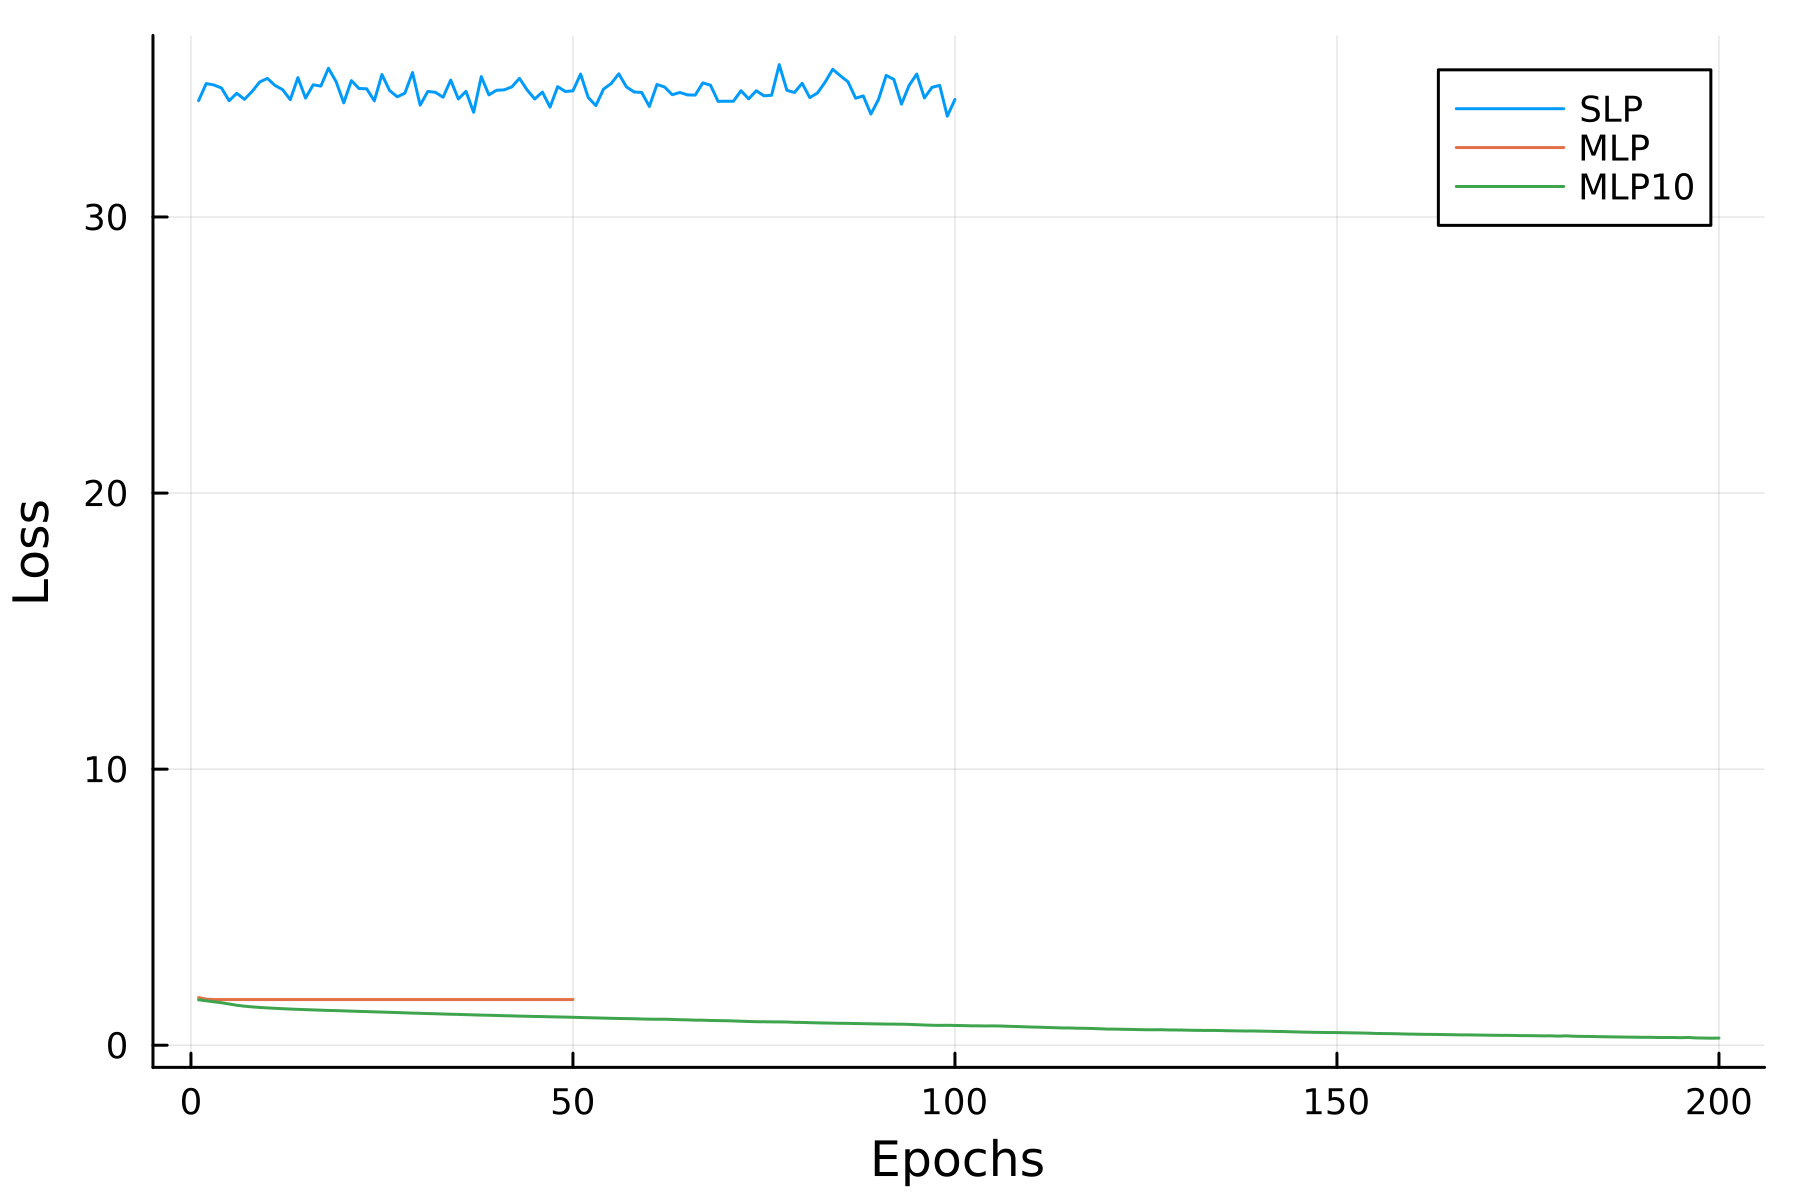
\includegraphics[width=\textwidth]{loss_plot_25_8}
        \caption{Training losses}
        \label{fig:loss}
    \end{subfigure}
    \end{minipage}
    \\
    \centering
    \begin{minipage}[b]{.6\textwidth}
    \begin{subfigure}[b]{\textwidth}
        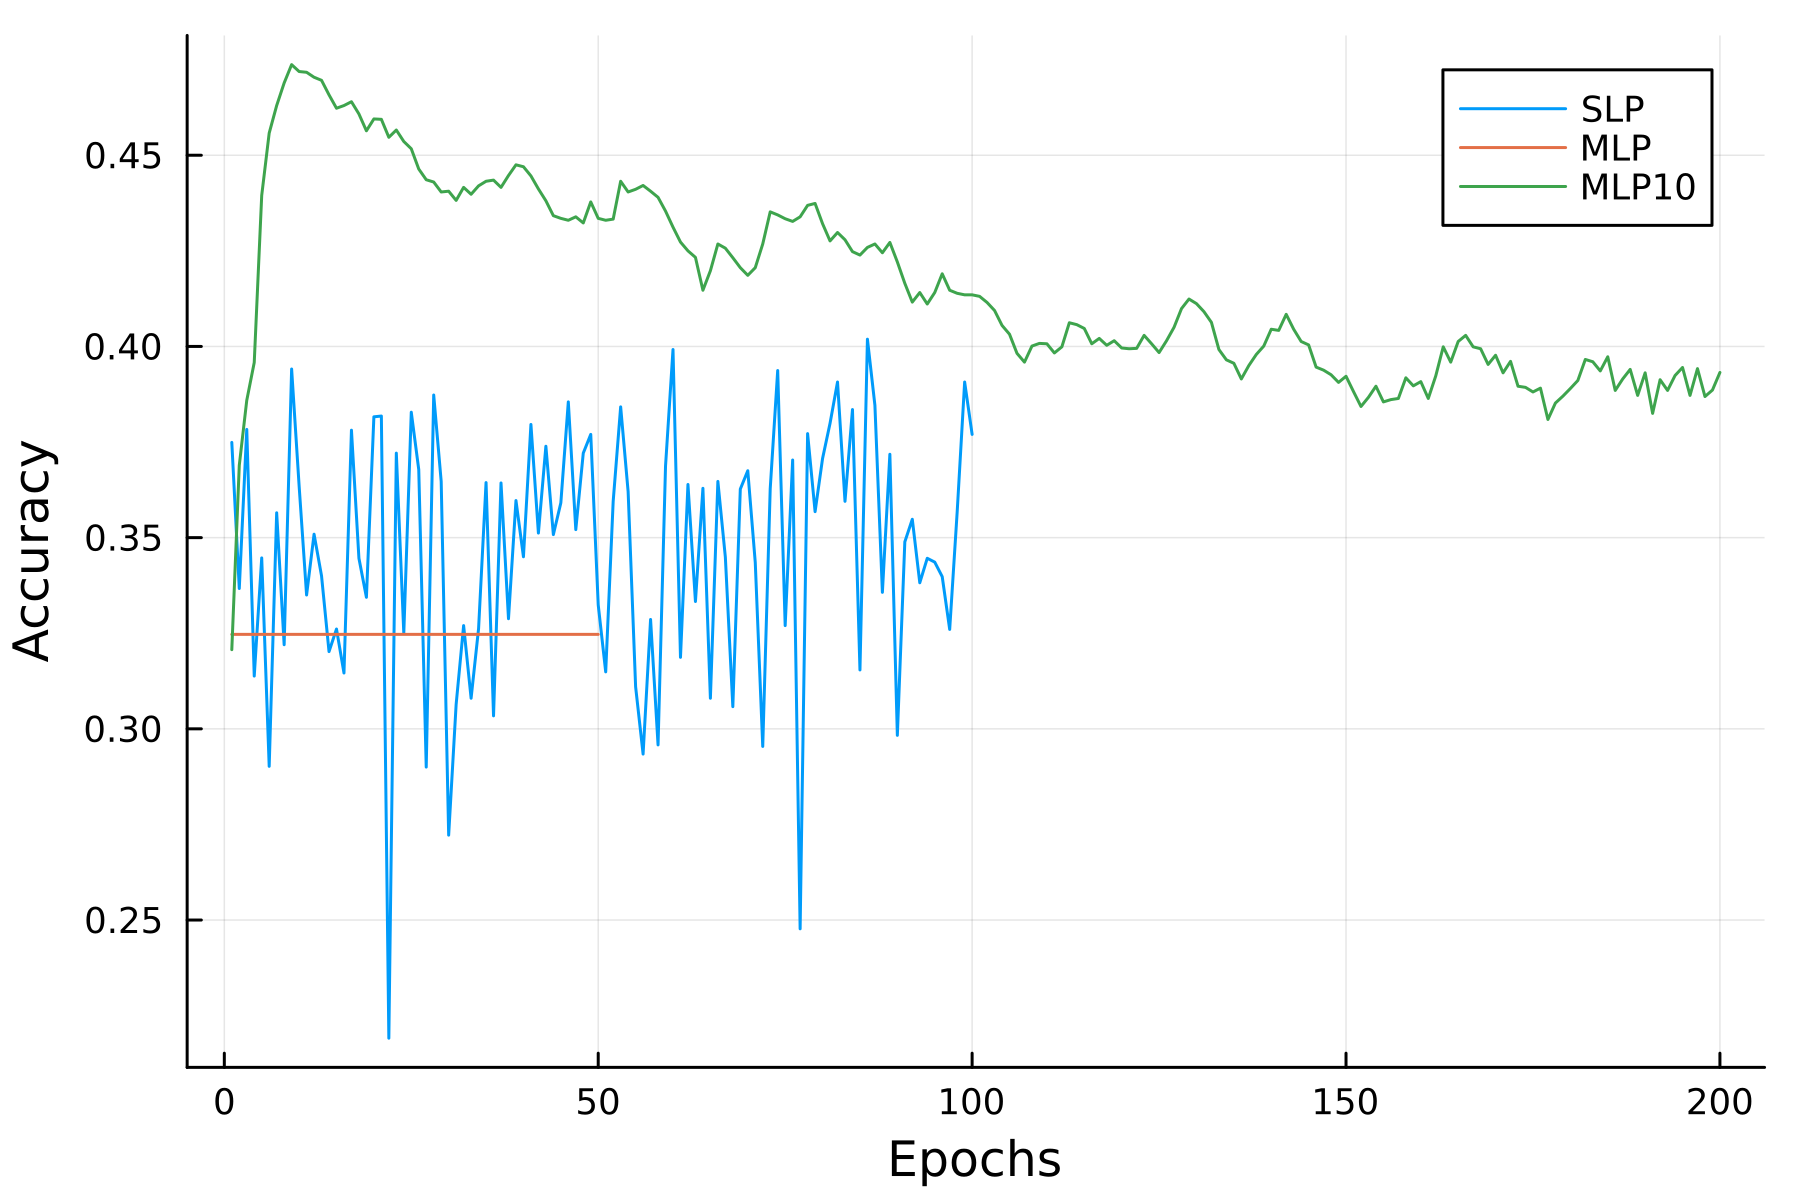
\includegraphics[width=\textwidth]{accuracy_plot_25_8}
        \caption{Accuracies}
        \label{fig:accuracy}
    \end{subfigure}
    \end{minipage}
    \\
    \centering
    \begin{minipage}[b]{.6\textwidth}
    \begin{subfigure}[b]{\textwidth}
        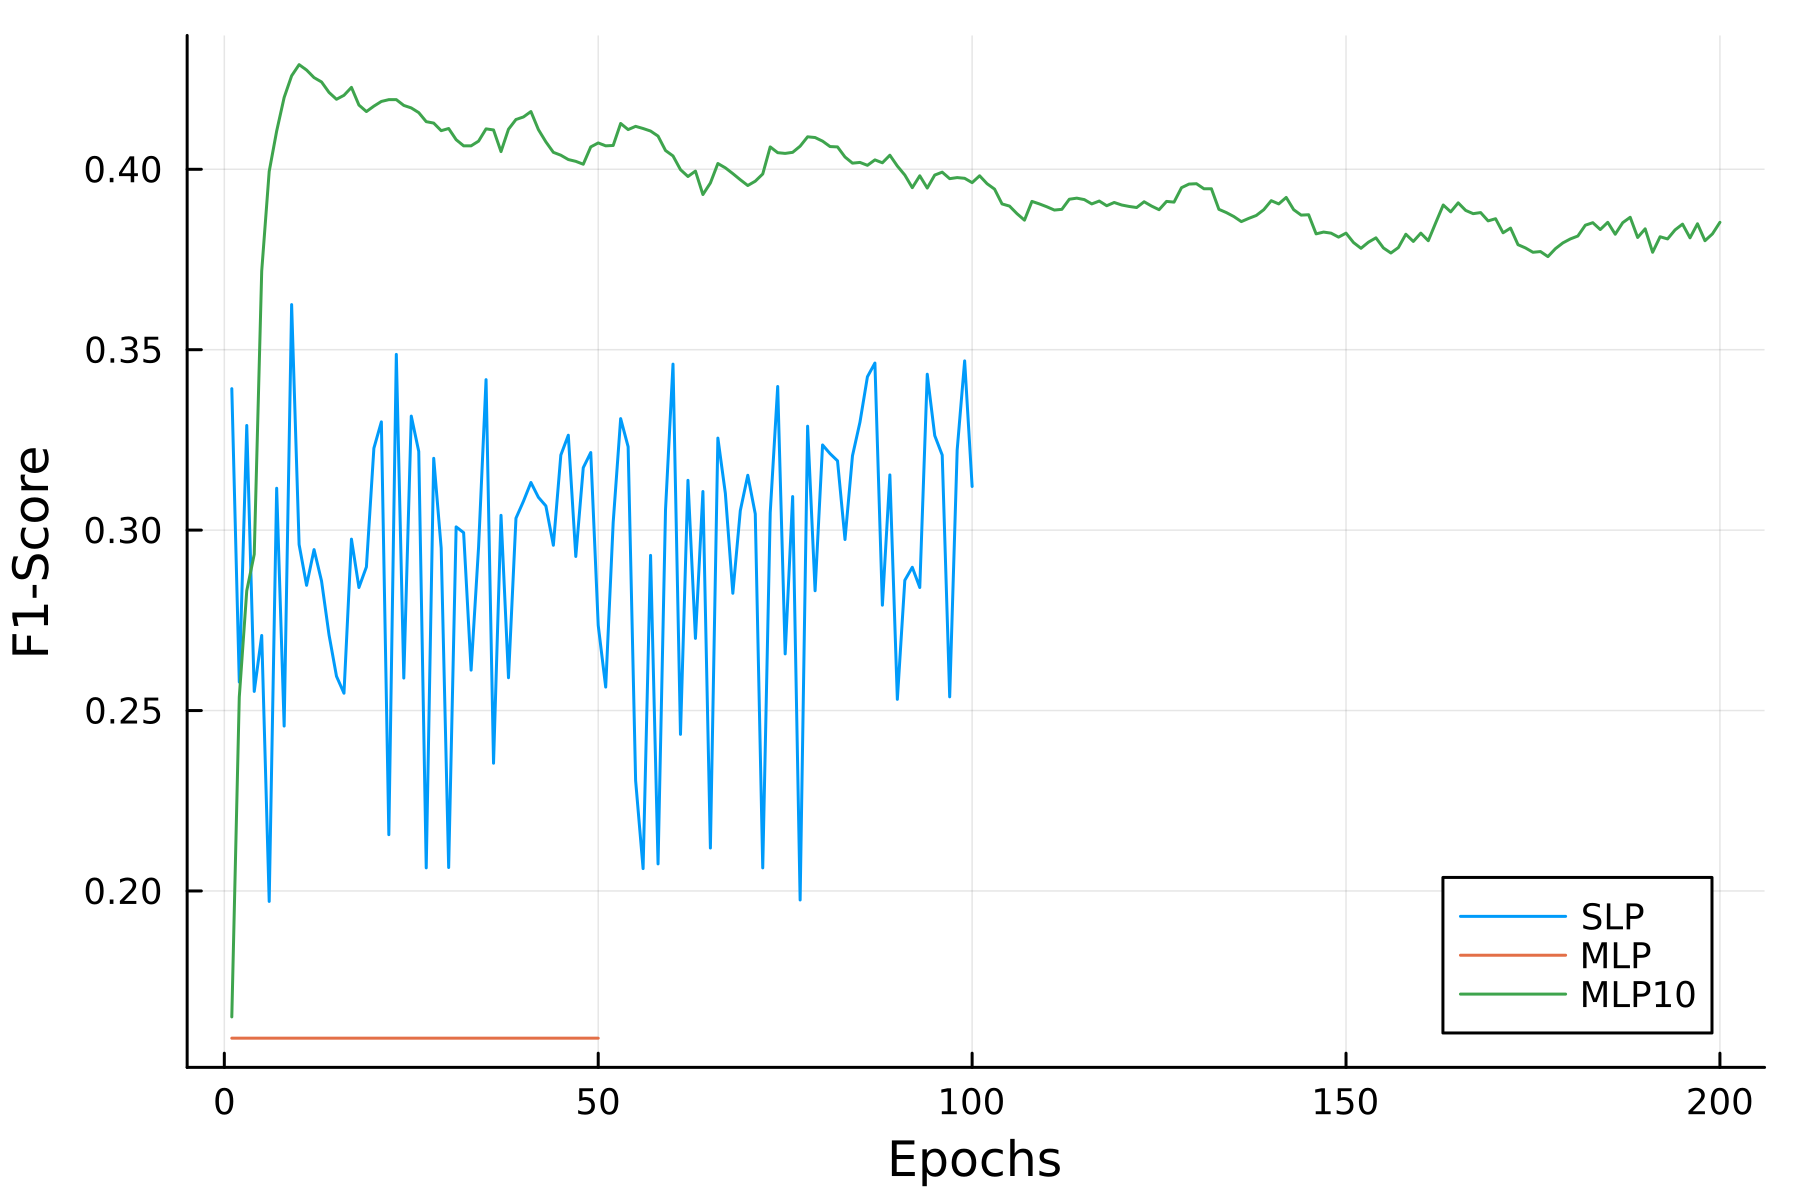
\includegraphics[width=\textwidth]{f1_plot_25_8}
        \caption{F1-scores}\label{fig:f1}
    \end{subfigure}
    \end{minipage}
    \caption{(a) cross-entropy losses (b) accuracies (c) F1-scores of all perceptron-based configurations tested. Trained with neighborhood-encodings of 60 \% of the training dataset of NetSurfP 2.0. Here $n=25$ and the secondary structure classification is dssp8-based. Note that the SLP and 1-layer MLP model was evaluated using fewer epochs than their 10-layer counterpart.}\label{fig:she2}
    \end{figure}

\begin{figure}[H]
        \centering
        \begin{minipage}[b]{.6\textwidth}
            \begin{subfigure}[b]{\textwidth}
            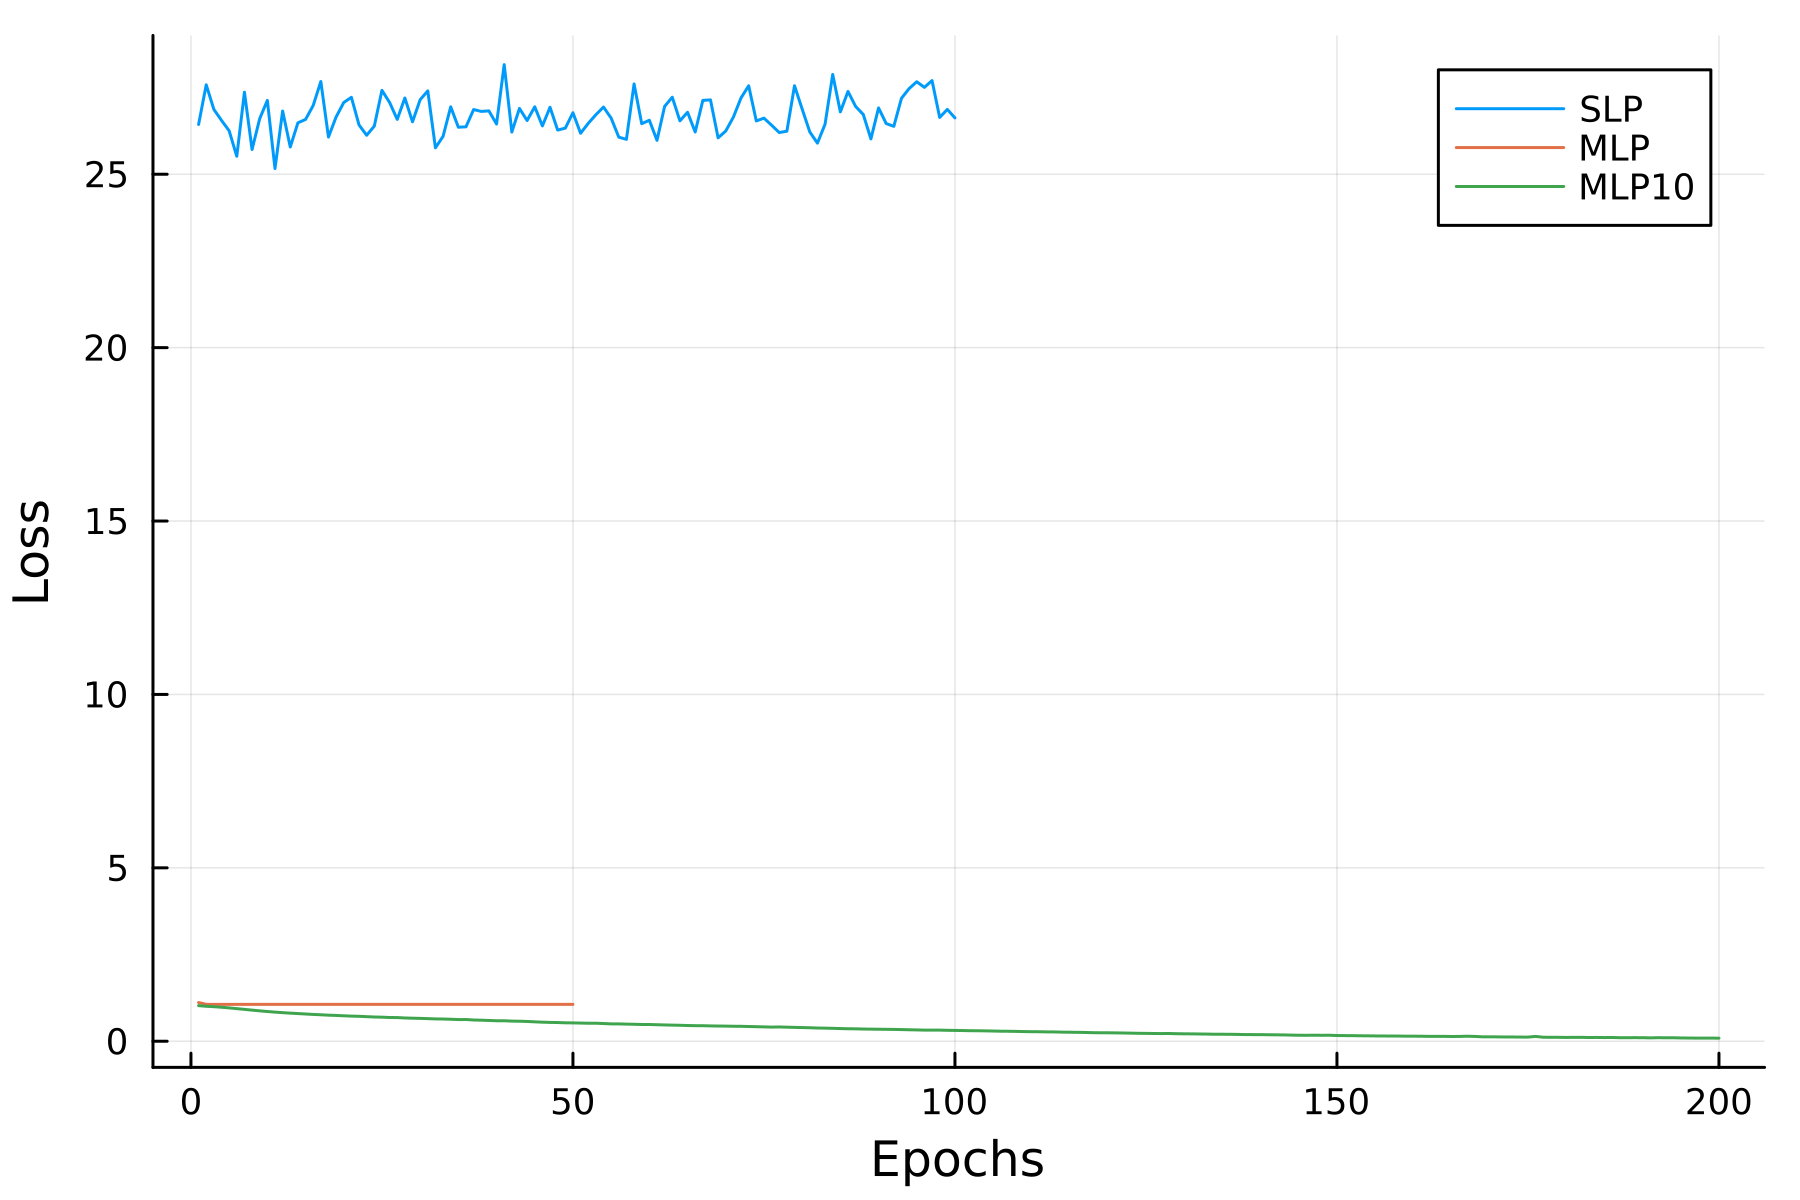
\includegraphics[width=\textwidth]{loss_plot_100_3}
            \caption{Training losses}
            \label{fig:loss}
        \end{subfigure}
        \end{minipage}
        \\
        \centering
        \begin{minipage}[b]{.6\textwidth}
        \begin{subfigure}[b]{\textwidth}
            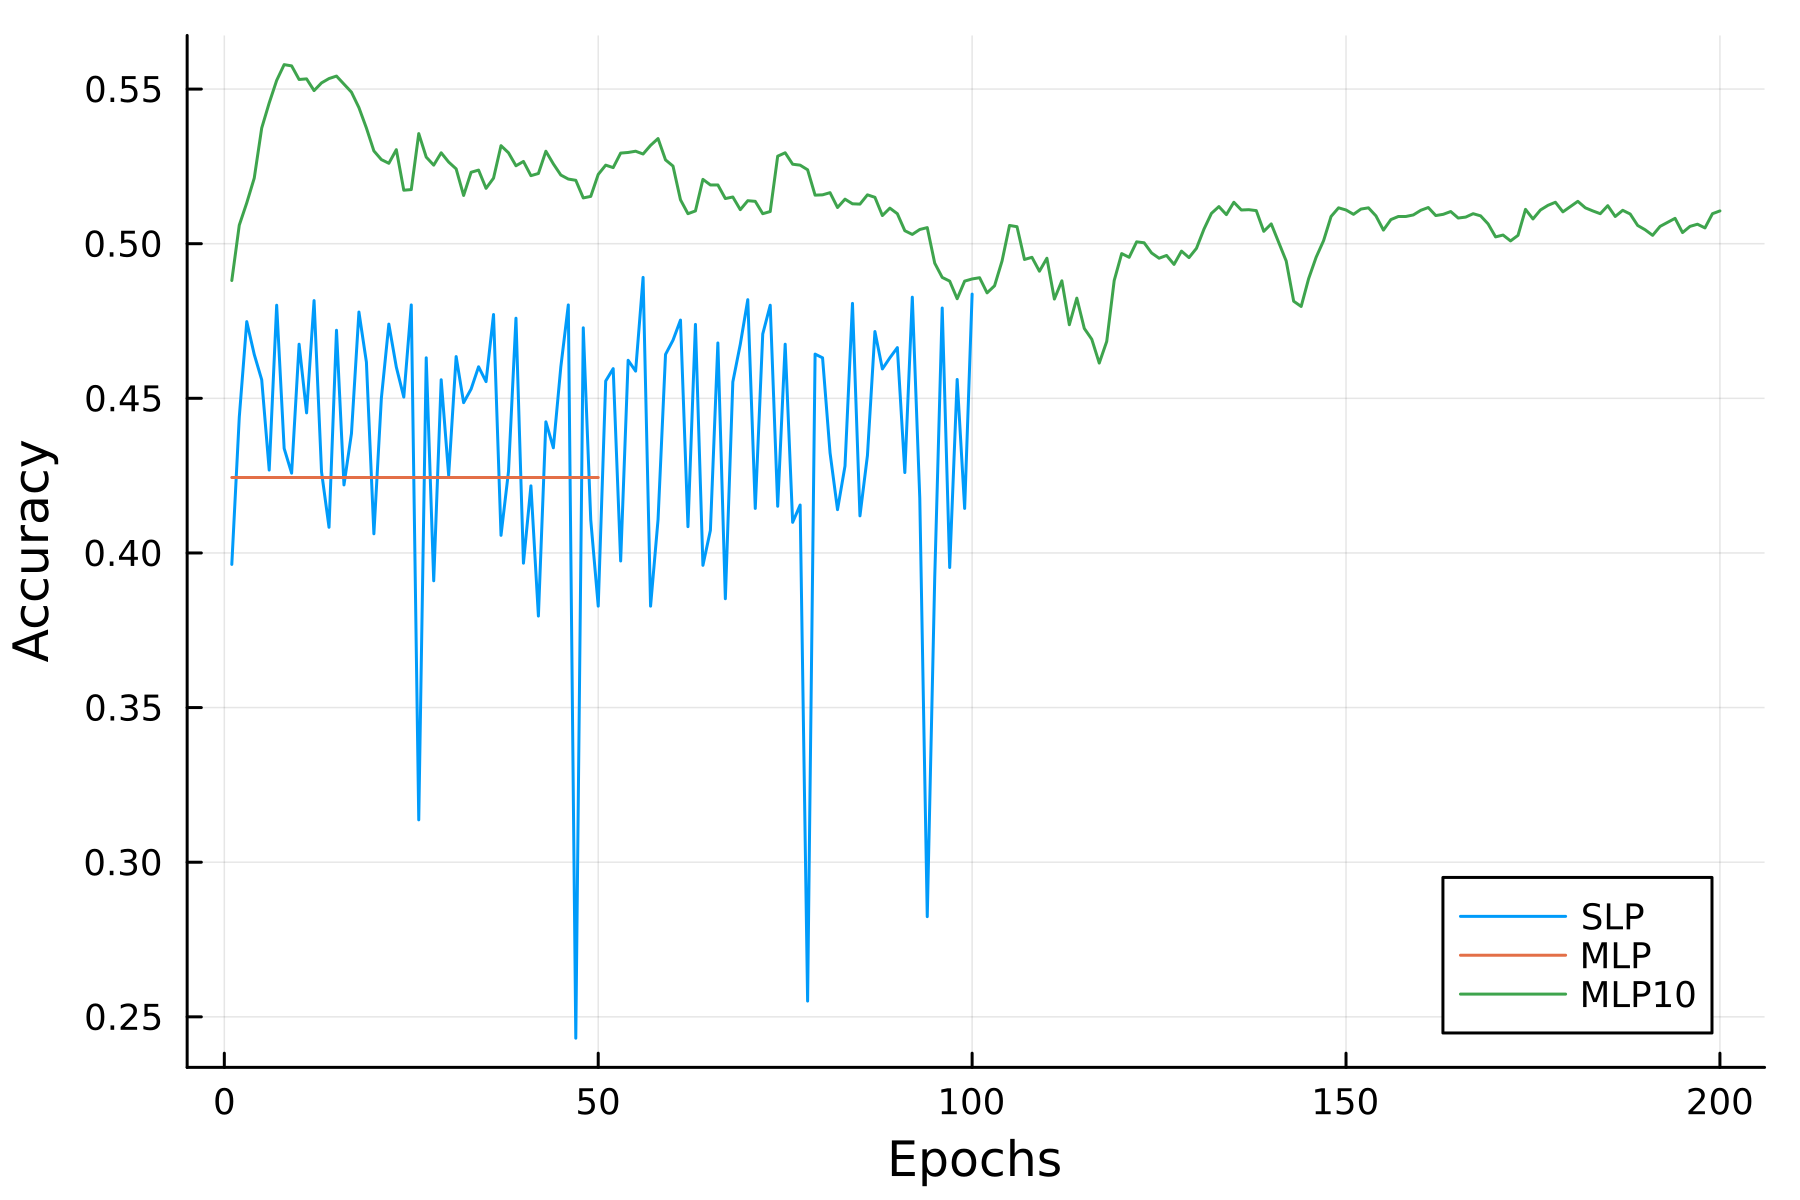
\includegraphics[width=\textwidth]{accuracy_plot_100_3}
            \caption{Accuracies}
            \label{fig:accuracy}
        \end{subfigure}
        \end{minipage}
        \\
        \centering
        \begin{minipage}[b]{.6\textwidth}
        \begin{subfigure}[b]{\textwidth}
            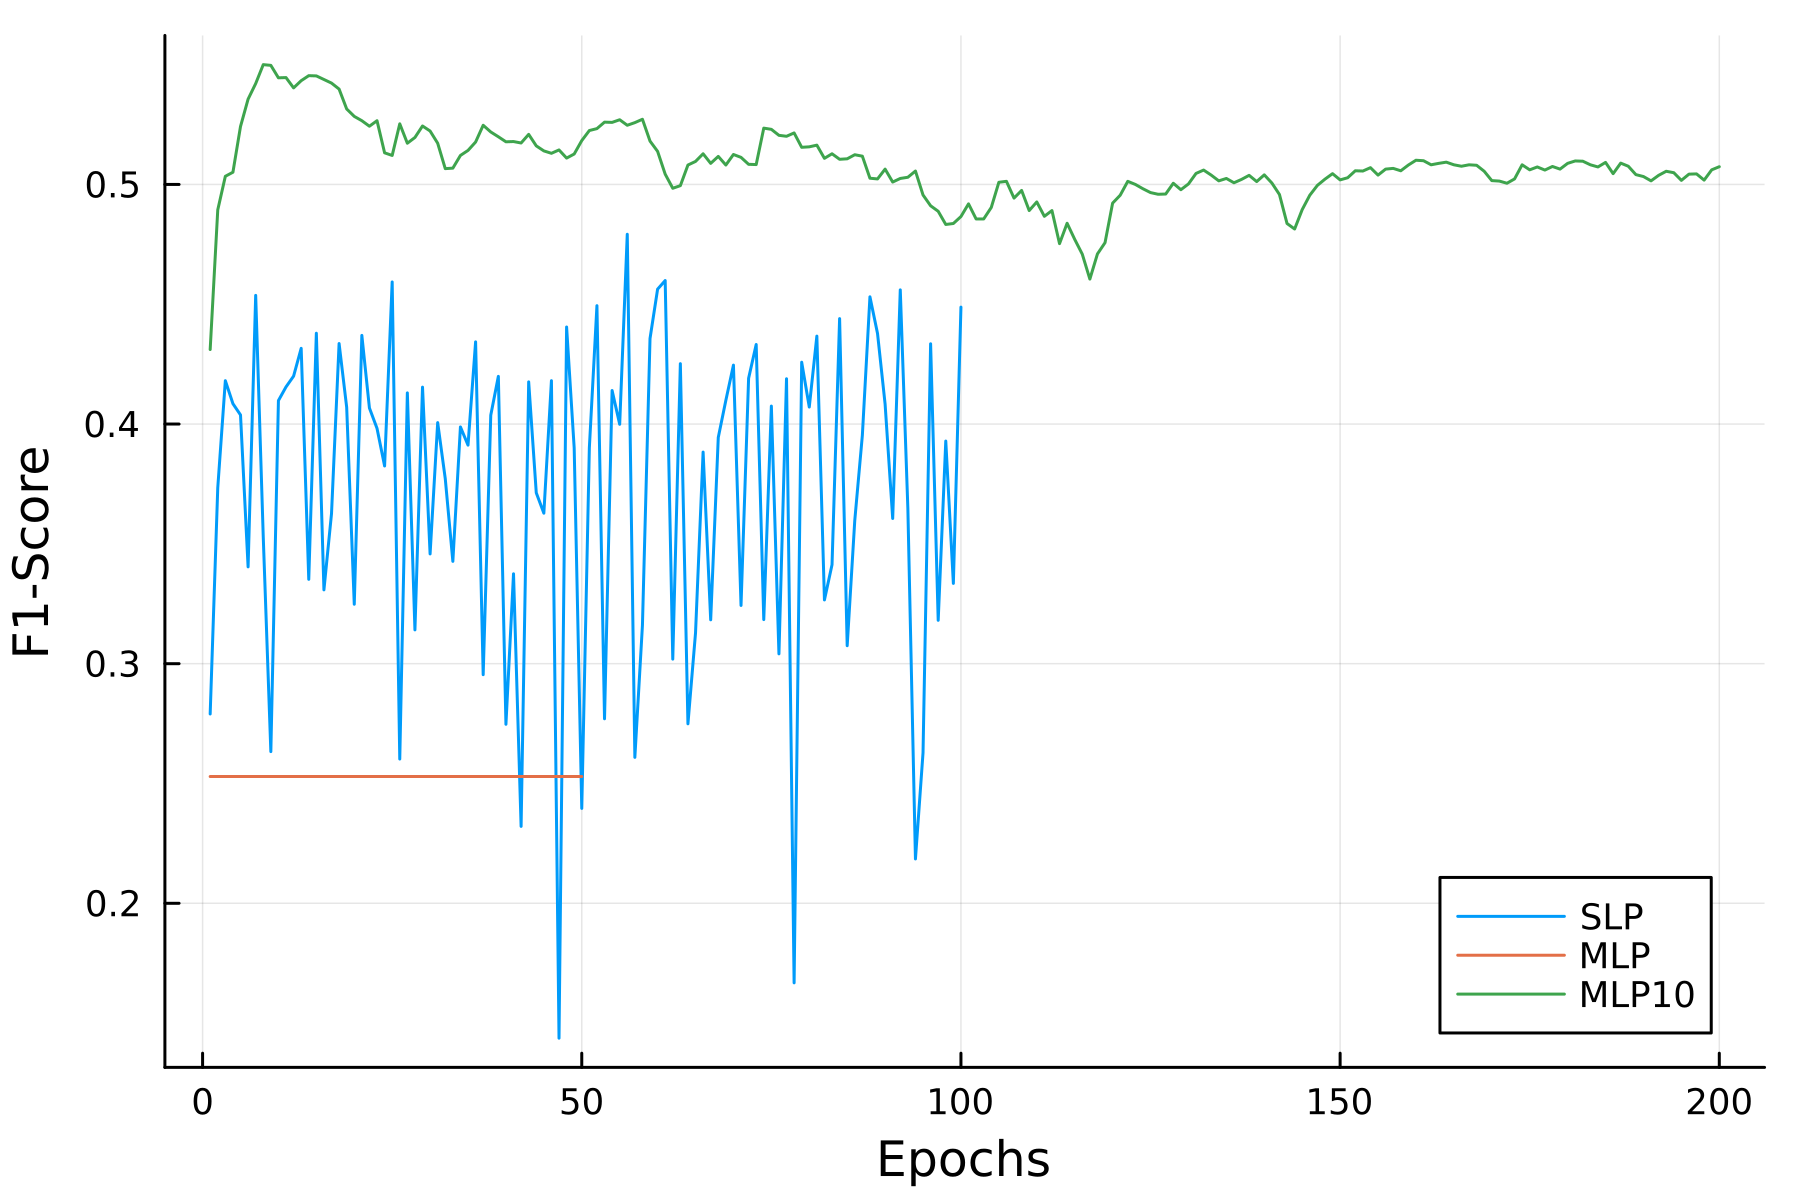
\includegraphics[width=\textwidth]{f1_plot_100_3}
            \caption{F1-scores}\label{fig:f1}
        \end{subfigure}
        \end{minipage}
        \caption{(a) cross-entropy losses (b) accuracies (c) F1-scores of all perceptron-based configurations tested. Trained with neighborhood-encodings of 60 \% of the training dataset of NetSurfP 2.0. Here $n=100$ and the secondary structure classification is dssp3-based. Note that the SLP and 1-layer MLP model was evaluated using fewer epochs than their 10-layer counterpart.}\label{fig:she3}
        \end{figure}

        \begin{figure}[H]
            \centering
            \begin{minipage}[b]{.6\textwidth}
                \begin{subfigure}[b]{\textwidth}
                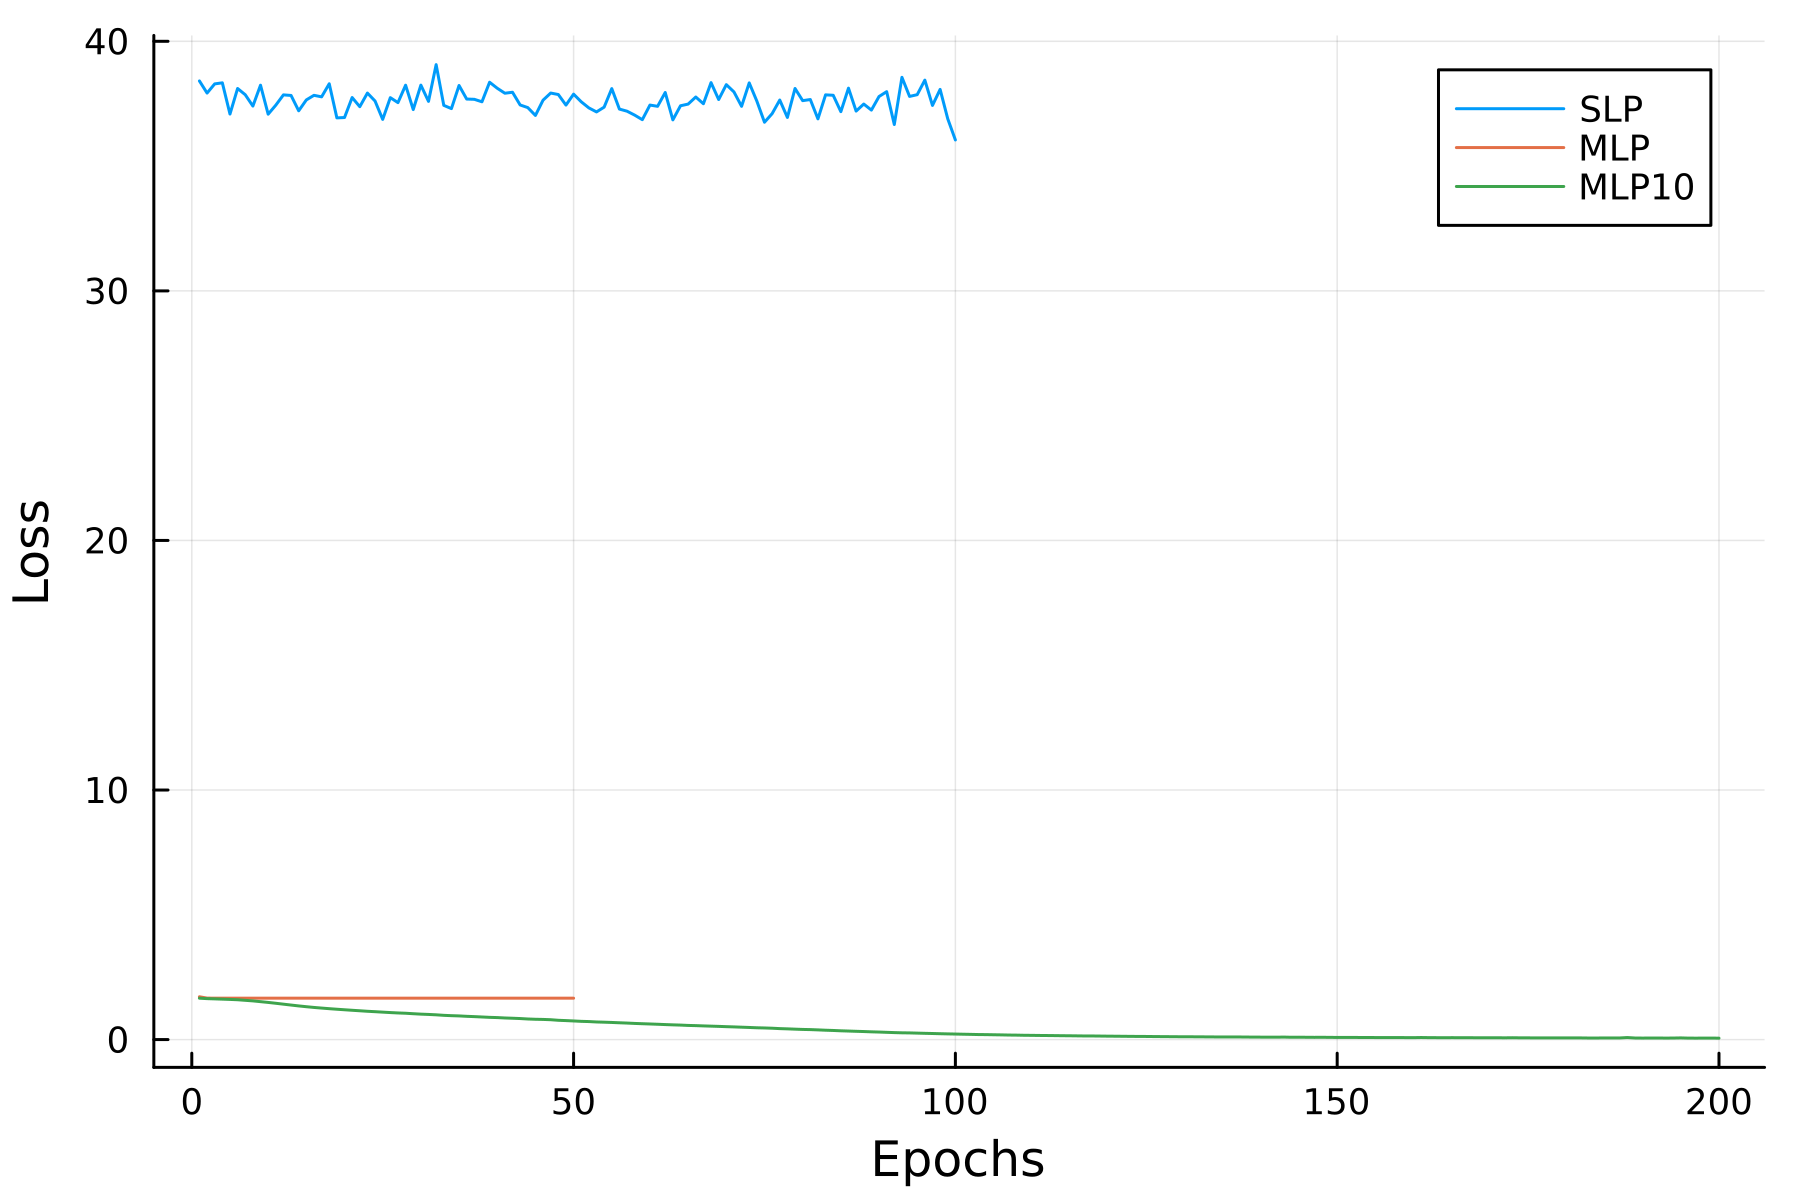
\includegraphics[width=\textwidth]{loss_plot_100_8}
                \caption{Training losses}
                \label{fig:loss}
            \end{subfigure}
            \end{minipage}
            \\
            \centering
            \begin{minipage}[b]{.6\textwidth}
            \begin{subfigure}[b]{\textwidth}
                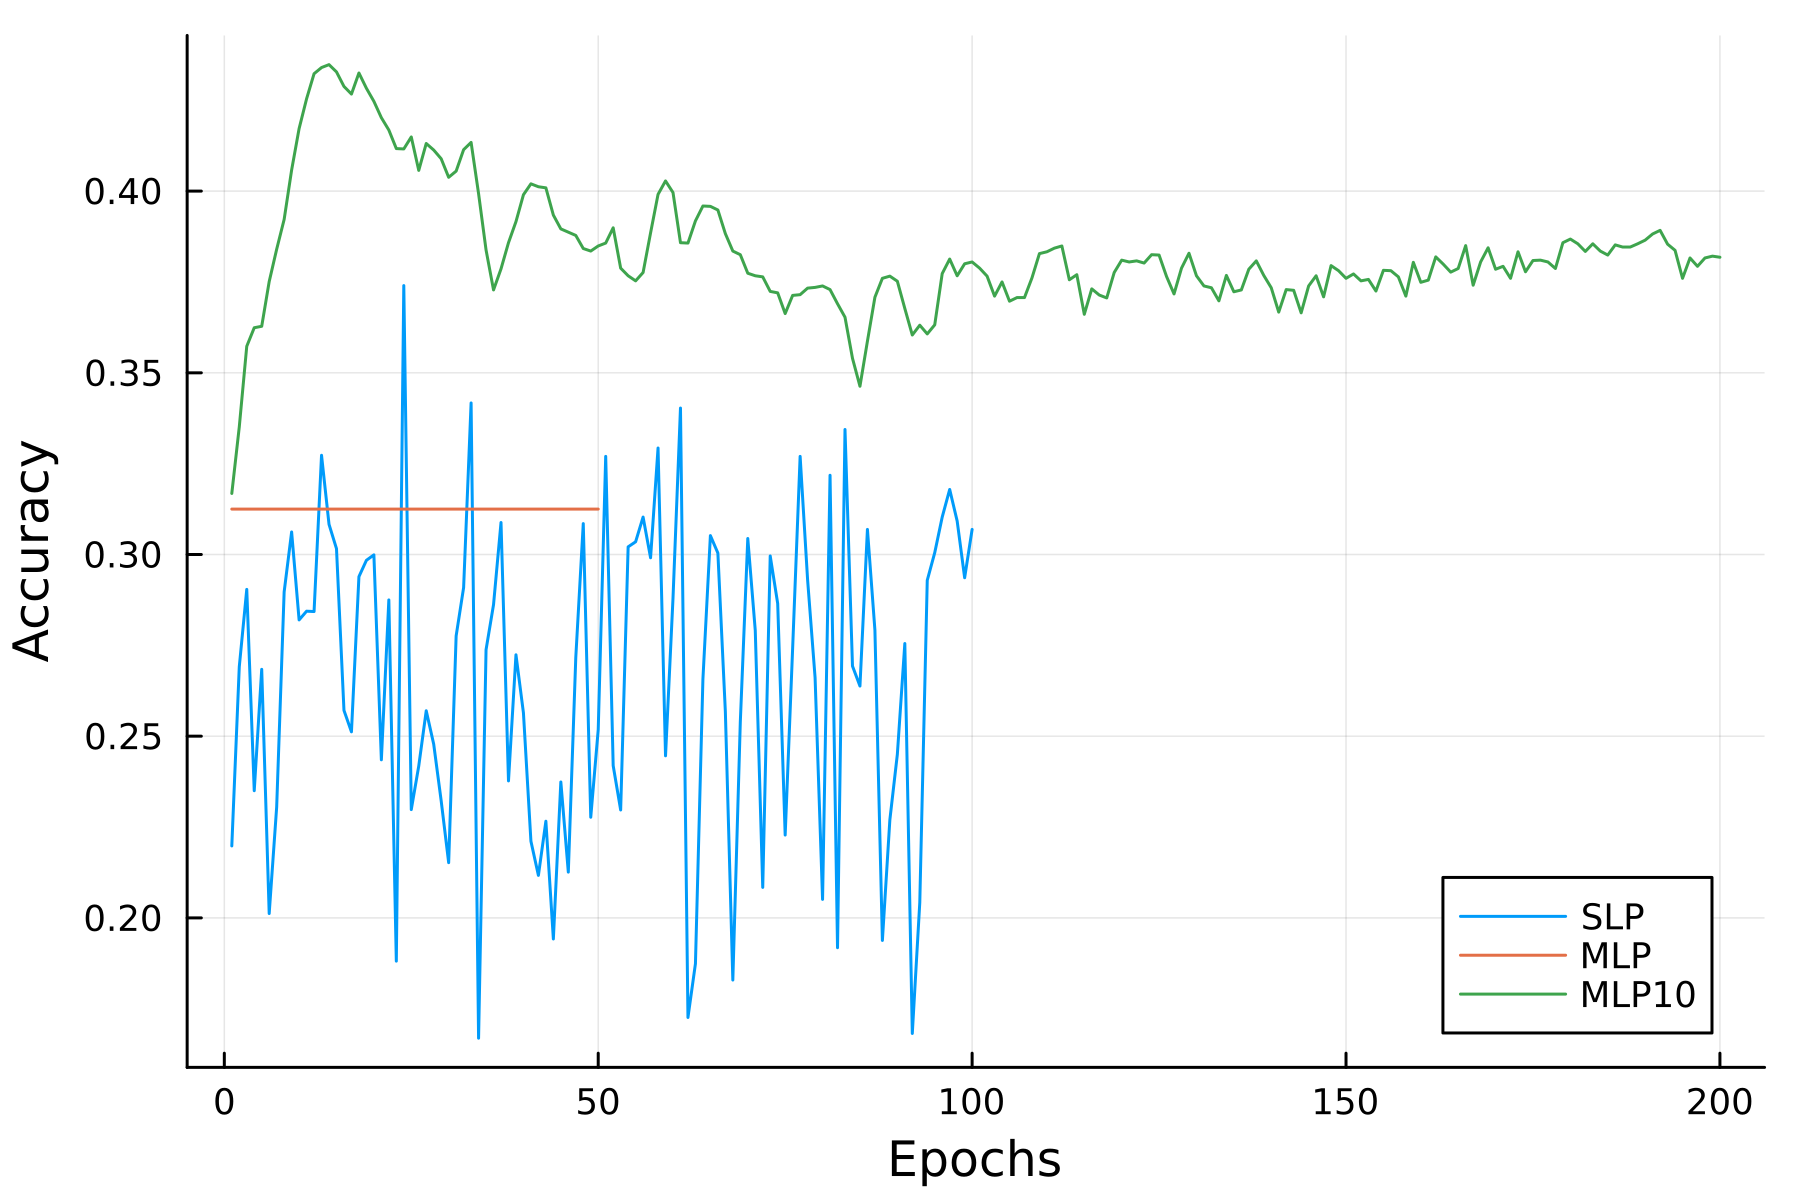
\includegraphics[width=\textwidth]{accuracy_plot_100_8}
                \caption{Accuracies}
                \label{fig:accuracy}
            \end{subfigure}
            \end{minipage}
            \\
            \centering
            \begin{minipage}[b]{.6\textwidth}
            \begin{subfigure}[b]{\textwidth}
                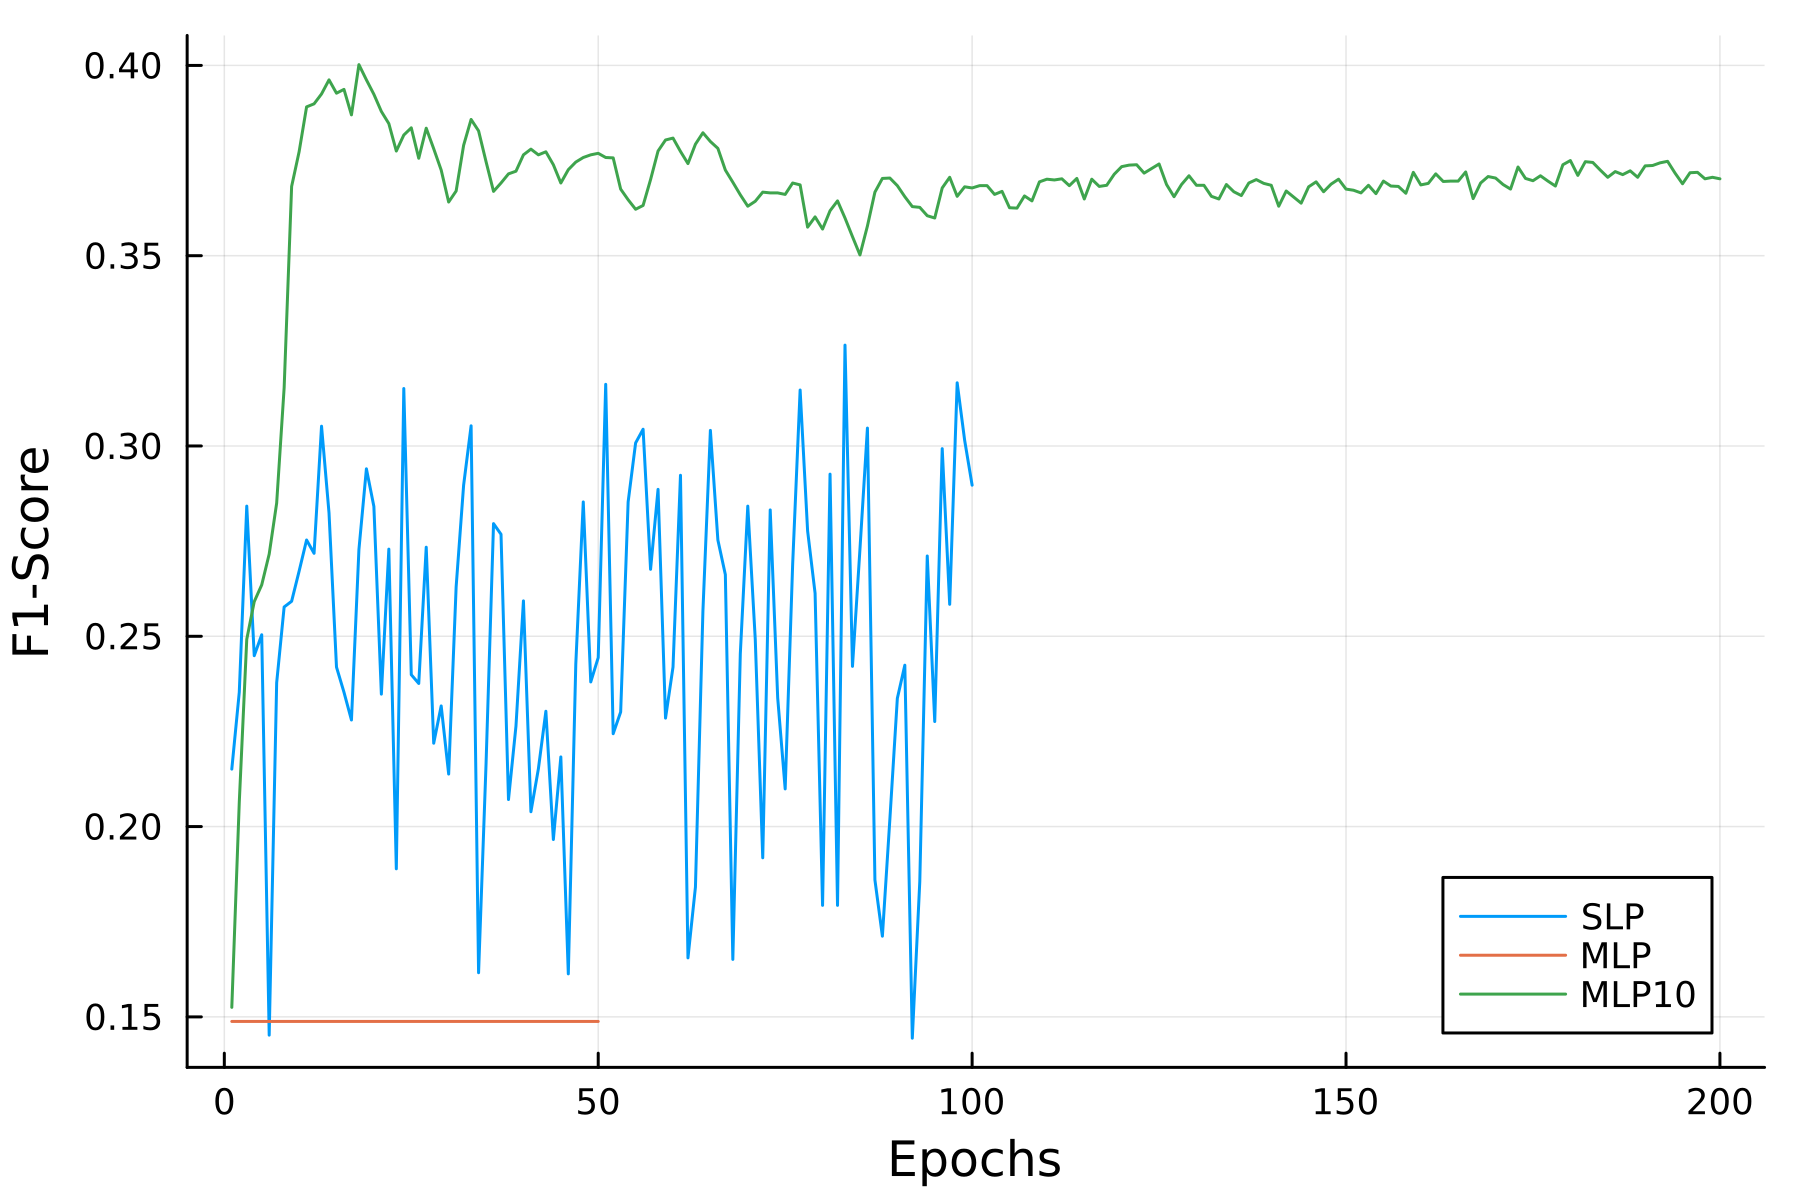
\includegraphics[width=\textwidth]{f1_plot_100_8}
                \caption{F1-scores}\label{fig:f1}
            \end{subfigure}
            \end{minipage}
            \caption{(a) cross-entropy losses (b) accuracies (c) F1-scores of all perceptron-based configurations tested. Trained with neighborhood-encodings of 60 \% of the training dataset of NetSurfP 2.0. Here $n=100$ and the secondary structure classification is dssp8-based. Note that the SLP and 1-layer MLP model was evaluated using fewer epochs than their 10-layer counterpart.}\label{fig:she4}
            \end{figure}

\end{appendices}

\end{document}
